% node_definitions.tex - Network node rendering and management
% This module defines how to create and render individual network assets

% ============================================================================
% NODE DATA STRUCTURES
% ============================================================================

% Node counter for auto-indexing
\newcounter{nodecount}

% ============================================================================
% HASH MAP IMPLEMENTATION FOR O(1) NODE LOOKUP
% ============================================================================
% This implementation uses pgfkeys to create a hash map for efficient node lookup
% by IP address, hostname, or node ID

% Initialize hash map storage
\pgfkeys{
    /nodemap/.cd,
    .unknown/.code={
        \pgfkeyssetvalue{\pgfkeyscurrentpath/\pgfkeyscurrentname}{#1}
    }
}

% Register a node in the hash map
% Usage: \registerNode{nodeID}{IP}{hostname}
\newcommand{\registerNode}[3]{
    % Store by node ID
    \pgfkeys{/nodemap/byid/#1/.initial={#1}}
    \pgfkeys{/nodemap/byid/#1/ip/.initial={#2}}
    \pgfkeys{/nodemap/byid/#1/hostname/.initial={#3}}

    % Store by IP address (replace . with _ for key safety)
    \StrSubstitute{#2}{.}{_}[\safeip]
    \pgfkeys{/nodemap/byip/\safeip/.initial={#1}}

    % Store by hostname
    \pgfkeys{/nodemap/byhost/#3/.initial={#1}}
}

% Lookup node ID by IP address
% Usage: \getNodeByIP{192.168.1.10}{\resultvar}
\newcommand{\getNodeByIP}[2]{
    \StrSubstitute{#1}{.}{_}[\safeip]
    \pgfkeysgetvalue{/nodemap/byip/\safeip}{#2}
}

% Lookup node ID by hostname
% Usage: \getNodeByHostname{webserver}{\resultvar}
\newcommand{\getNodeByHostname}[2]{
    \pgfkeysgetvalue{/nodemap/byhost/#1}{#2}
}

% Get node IP by node ID
% Usage: \getNodeIP{srv1}{\resultvar}
\newcommand{\getNodeIP}[2]{
    \pgfkeysgetvalue{/nodemap/byid/#1/ip}{#2}
}

% Get node hostname by node ID
% Usage: \getNodeHostname{srv1}{\resultvar}
\newcommand{\getNodeHostname}[2]{
    \pgfkeysgetvalue{/nodemap/byid/#1/hostname}{#2}
}

% ============================================================================
% EXTENDED HASH MAP WITH METADATA STORAGE
% ============================================================================

% Register node with extended metadata
% Usage: \registerNodeExtended{nodeID}{IP}{hostname}{type}{os}{status}
\newcommand{\registerNodeExtended}[6]{
    % Basic registration
    \registerNode{#1}{#2}{#3}

    % Extended metadata
    \pgfkeys{/nodemap/byid/#1/type/.initial={#4}}
    \pgfkeys{/nodemap/byid/#1/os/.initial={#5}}
    \pgfkeys{/nodemap/byid/#1/status/.initial={#6}}
}

% Store node group/cluster membership
% Usage: \assignNodeToCluster{nodeID}{clusterID}
\newcommand{\assignNodeToCluster}[2]{
    \pgfkeys{/nodemap/byid/#1/cluster/.initial={#2}}
}

% Store parent-child relationship (for VMs, containers)
% Usage: \setNodeParent{nodeID}{parentID}
\newcommand{\setNodeParent}[2]{
    \pgfkeys{/nodemap/byid/#1/parent/.initial={#2}}
}

% Store node services
% Usage: \setNodeServices{nodeID}{services}
\newcommand{\setNodeServices}[2]{
    \pgfkeys{/nodemap/byid/#1/services/.initial={#2}}
}

% Store node security status
% Usage: \setNodeSecurity{nodeID}{vulncount}{cvss}{compliance}
\newcommand{\setNodeSecurity}[4]{
    \pgfkeys{/nodemap/byid/#1/vulncount/.initial={#2}}
    \pgfkeys{/nodemap/byid/#1/cvss/.initial={#3}}
    \pgfkeys{/nodemap/byid/#1/compliance/.initial={#4}}
}

% Get node metadata
\newcommand{\getNodeType}[2]{
    \pgfkeysgetvalue{/nodemap/byid/#1/type}{#2}
}

\newcommand{\getNodeOS}[2]{
    \pgfkeysgetvalue{/nodemap/byid/#1/os}{#2}
}

\newcommand{\getNodeStatus}[2]{
    \pgfkeysgetvalue{/nodemap/byid/#1/status}{#2}
}

\newcommand{\getNodeCluster}[2]{
    \pgfkeysgetvalue{/nodemap/byid/#1/cluster}{#2}
}

\newcommand{\getNodeParent}[2]{
    \pgfkeysgetvalue{/nodemap/byid/#1/parent}{#2}
}

% TODO: Advanced hash map features
% - Index nodes by multiple attributes simultaneously
% - Support for node tagging and label querying
% - Network topology graph representation

% ============================================================================
% IP ADDRESS VALIDATION AND FORMATTING
% ============================================================================

% Validate IPv4 address format
% Usage: \validateIPv4{192.168.1.10}{\resultvar}
% Result: 1 if valid, 0 if invalid
\newcommand{\validateIPv4}[2]{
    \def#2{1} % Assume valid by default

    % Check if IP contains 3 dots
    \StrCount{#1}{.}[\dotcount]
    \ifnum\dotcount=3\relax
        % Valid format (basic check)
        \def#2{1}
    \else
        \def#2{0}
    \fi
}

% Validate IPv6 address format (basic check)
% Usage: \validateIPv6{2001:0db8::1}{\resultvar}
% Result: 1 if valid, 0 if invalid
\newcommand{\validateIPv6}[2]{
    \def#2{1} % Assume valid by default

    % Check if IP contains colons
    \StrCount{#1}{:}[\coloncount]
    \ifnum\coloncount>1\relax
        % Valid format (basic check)
        \def#2{1}
    \else
        \def#2{0}
    \fi
}

% Auto-detect IP version and validate
% Usage: \validateIP{192.168.1.10}{\resultvar}
% Result: 4 for IPv4, 6 for IPv6, 0 for invalid
\newcommand{\validateIP}[2]{
    \StrCount{#1}{.}[\dotcount]
    \StrCount{#1}{:}[\coloncount]

    \ifnum\dotcount=3\relax
        \def#2{4} % IPv4
    \else
        \ifnum\coloncount>1\relax
            \def#2{6} % IPv6
        \else
            \def#2{0} % Invalid
        \fi
    \fi
}

% Format IP address with CIDR notation
% Usage: \formatCIDR{192.168.1.0}{24}{\resultvar}
\newcommand{\formatCIDR}[3]{
    \def#3{#1/#2}
}

% Extract subnet from IP address
% Usage: \extractSubnet{192.168.1.100}{\resultvar}
% Returns: 192.168.1.0 (class C subnet)
\newcommand{\extractSubnet}[2]{
    \StrCut{#1}{.}{\octetA}{\remaining}
    \StrCut{\remaining}{.}{\octetB}{\remaining}
    \StrCut{\remaining}{.}{\octetC}{\octetD}
    \def#2{\octetA.\octetB.\octetC.0}
}

% Determine if two IPs are in same subnet (simple /24 check)
% Usage: \sameSubnet{192.168.1.10}{192.168.1.20}{\resultvar}
% Result: 1 if same subnet, 0 if different
\newcommand{\sameSubnet}[3]{
    \extractSubnet{#1}{\subnetA}
    \extractSubnet{#2}{\subnetB}

    \ifthenelse{\equal{\subnetA}{\subnetB}}{
        \def#3{1}
    }{
        \def#3{0}
    }
}

% Validate IPv4 octet is in range 0-255
% Usage: \validateOctet{value}{\resultvar}
\newcommand{\validateOctet}[2]{
    \ifnum#1<0\relax
        \def#2{0}
    \else
        \ifnum#1>255\relax
            \def#2{0}
        \else
            \def#2{1}
        \fi
    \fi
}

% Enhanced IPv4 validation with octet range checking
% Usage: \validateIPv4Enhanced{192.168.1.10}{\resultvar}
\newcommand{\validateIPv4Enhanced}[2]{
    \def#2{0} % Assume invalid by default

    % First check format
    \StrCount{#1}{.}[\dotcount]
    \ifnum\dotcount=3\relax
        % Extract octets
        \StrCut{#1}{.}{\octetA}{\remaining}
        \StrCut{\remaining}{.}{\octetB}{\remaining}
        \StrCut{\remaining}{.}{\octetC}{\octetD}

        % Note: Full range validation would require more complex LaTeX programming
        % This is a basic structure - full implementation would need numeric comparison
        \def#2{1} % Mark as valid if format is correct
    \fi
}

% Extract subnet with variable CIDR prefix
% Usage: \extractSubnetCIDR{192.168.1.100}{24}{\resultvar}
\newcommand{\extractSubnetCIDR}[3]{
    \StrCut{#1}{.}{\octetA}{\remaining}
    \StrCut{\remaining}{.}{\octetB}{\remaining}
    \StrCut{\remaining}{.}{\octetC}{\octetD}

    \ifnum#2=8\relax
        \def#3{\octetA.0.0.0}
    \else
        \ifnum#2=16\relax
            \def#3{\octetA.\octetB.0.0}
        \else
            \ifnum#2=24\relax
                \def#3{\octetA.\octetB.\octetC.0}
            \else
                % Default to /24
                \def#3{\octetA.\octetB.\octetC.0}
            \fi
        \fi
    \fi
}

% Check if IP is in private range
% Usage: \isPrivateIP{192.168.1.10}{\resultvar}
% Returns: 1 if private, 0 if public
\newcommand{\isPrivateIP}[2]{
    \StrCut{#1}{.}{\octetA}{\remaining}
    \StrCut{\remaining}{.}{\octetB}{\remaining}

    % Check for 10.0.0.0/8
    \ifthenelse{\equal{\octetA}{10}}{
        \def#2{1}
    }{
    % Check for 192.168.0.0/16
    \ifthenelse{\equal{\octetA}{192}}{
        \ifthenelse{\equal{\octetB}{168}}{
            \def#2{1}
        }{
            \def#2{0}
        }
    }{
    % Check for 172.16.0.0/12 (172.16-172.31)
    \ifthenelse{\equal{\octetA}{172}}{
        \def#2{1} % Simplified - should check 16-31 range
    }{
        \def#2{0}
    }}}
}

% TODO: Advanced IP validation
% - Full numeric range validation for octets (requires lua or complex TeX)
% - Full IPv6 validation with compression
% - CIDR validation and calculations
% - IP range validation (start-end)

% ============================================================================
% BASIC NODE CREATION COMMANDS
% ============================================================================

% Create a server node
% Usage: \createServer{name}{ip}{x}{y}{label}
\newcommand{\createServer}[5]{
    \node[server] (#1) at (#3,#4) {
        \textbf{#5} \\[2pt]
        \tikz\node[ip label]{#2};
    };
}

% Create a client node
% Usage: \createClient{name}{ip}{x}{y}{label}
\newcommand{\createClient}[5]{
    \node[client] (#1) at (#3,#4) {
        \textbf{#5} \\[2pt]
        \tikz\node[ip label]{#2};
    };
}

% Create a router node
% Usage: \createRouter{name}{ip}{x}{y}{label}
\newcommand{\createRouter}[5]{
    \node[router] (#1) at (#3,#4) {
        \textbf{#5} \\[2pt]
        \tikz\node[ip label]{#2};
    };
}

% Create a firewall node
% Usage: \createFirewall{name}{ip}{x}{y}{label}
\newcommand{\createFirewall}[5]{
    \node[firewall] (#1) at (#3,#4) {
        \textbf{#5} \\[2pt]
        \tikz\node[ip label]{#2};
    };
}

% Create a switch node
% Usage: \createSwitch{name}{ip}{x}{y}{label}
\newcommand{\createSwitch}[5]{
    \node[switch] (#1) at (#3,#4) {
        \textbf{#5} \\[2pt]
        \tikz\node[ip label]{#2};
    };
}

% Create a cloud/internet node
% Usage: \createCloud{name}{x}{y}{label}
\newcommand{\createCloud}[4]{
    \node[cloud] (#1) at (#2,#3) {
        \textbf{#4}
    };
}

% Create an attacker node
% Usage: \createAttacker{name}{ip}{x}{y}{label}
\newcommand{\createAttacker}[5]{
    \node[attacker] (#1) at (#3,#4) {
        \textbf{#5} \\[2pt]
        \tikz\node[ip label, fill=threatCritical!20]{#2};
    };
}

% TODO: Advanced node creation
% - Add support for custom node shapes via parameters
% - Implement node templates for common device types
% - Add automatic IP validation and formatting
% - Create composite nodes (e.g., server rack with multiple servers)
% - Support for node status indicators (up/down/warning)

% ============================================================================
% ENHANCED NODE VARIANTS
% ============================================================================

% Create a server with port information
% Usage: \createServerWithPorts{name}{ip}{x}{y}{label}{ports}
\newcommand{\createServerWithPorts}[6]{
    \node[server, minimum height=2cm] (#1) at (#3,#4) {
        \textbf{#5} \\[2pt]
        \tikz\node[ip label]{#2}; \\[3pt]
        \tikz\node[port label]{#6};
    };
}

% Create a node with security status indicator
% Usage: \createSecureNode{type}{name}{ip}{x}{y}{label}{status}
% Status: secure, warning, compromised
\newcommand{\createSecureNode}[7]{
    \ifthenelse{\equal{#7}{secure}}{
        \def\statuscolor{clientGreen}
    }{
    \ifthenelse{\equal{#7}{warning}}{
        \def\statuscolor{threatMedium}
    }{
        \def\statuscolor{threatCritical}
    }}
    
    \ifthenelse{\equal{#1}{server}}{
        \createServer{#2}{#3}{#4}{#5}{#6}
    }{
    \ifthenelse{\equal{#1}{client}}{
        \createClient{#2}{#3}{#4}{#5}{#6}
    }{
        \createServer{#2}{#3}{#4}{#5}{#6}
    }}
    
    \node[circle, fill=\statuscolor, inner sep=2pt, 
          anchor=north east] at (#2.north east) {};
}

% ============================================================================
% DATABASE SERVER NODES
% ============================================================================

% Create a database server node (basic)
% Usage: \createDatabase{name}{ip}{x}{y}{label}
\newcommand{\createDatabase}[5]{
    \node[database] (#1) at (#3,#4) {
        \textbf{#5} \\[2pt]
        \tikz\node[ip label]{#2};
    };
}

% Create a primary database server node
% Usage: \createDatabasePrimary{name}{ip}{x}{y}{label}
\newcommand{\createDatabasePrimary}[5]{
    \node[database primary] (#1) at (#3,#4) {
        \textbf{#5} \\[2pt]
        \tikz\node[ip label]{#2}; \\[1pt]
        \tikz\node[font=\tiny\bfseries, text=databaseTeal!90]{PRIMARY};
    };
}

% Create a replica database server node
% Usage: \createDatabaseReplica{name}{ip}{x}{y}{label}
\newcommand{\createDatabaseReplica}[5]{
    \node[database replica] (#1) at (#3,#4) {
        \textbf{#5} \\[2pt]
        \tikz\node[ip label]{#2}; \\[1pt]
        \tikz\node[font=\tiny\bfseries, text=databaseTeal!70]{REPLICA};
    };
}

% Create a cluster database server node
% Usage: \createDatabaseCluster{name}{ip}{x}{y}{label}
\newcommand{\createDatabaseCluster}[5]{
    \node[database cluster] (#1) at (#3,#4) {
        \textbf{#5} \\[2pt]
        \tikz\node[ip label]{#2}; \\[1pt]
        \tikz\node[font=\tiny\bfseries, text=databaseTeal!85]{CLUSTER};
    };
}

% ============================================================================
% LOAD BALANCER NODES
% ============================================================================

% Create a load balancer node (basic)
% Usage: \createLoadBalancer{name}{ip}{x}{y}{label}
\newcommand{\createLoadBalancer}[5]{
    \node[loadbalancer] (#1) at (#3,#4) {
        \textbf{#5} \\[2pt]
        \tikz\node[ip label]{#2};
    };
}

% Create an active load balancer node
% Usage: \createLoadBalancerActive{name}{ip}{x}{y}{label}{algorithm}
% Algorithm: round-robin, least-conn, ip-hash, weighted
\newcommand{\createLoadBalancerActive}[6]{
    \node[loadbalancer active] (#1) at (#3,#4) {
        \textbf{#5} \\[2pt]
        \tikz\node[ip label]{#2}; \\[1pt]
        \tikz\node[font=\tiny\ttfamily, text=loadBalancerCyan!90]{#6}; \\[1pt]
        \tikz\node[font=\tiny\bfseries, text=clientGreen!80]{ACTIVE};
    };
}

% Create a passive load balancer node
% Usage: \createLoadBalancerPassive{name}{ip}{x}{y}{label}
\newcommand{\createLoadBalancerPassive}[5]{
    \node[loadbalancer passive] (#1) at (#3,#4) {
        \textbf{#5} \\[2pt]
        \tikz\node[ip label]{#2}; \\[1pt]
        \tikz\node[font=\tiny\bfseries, text=black!50]{STANDBY};
    };
}

% Add load distribution indicator to load balancer
% Usage: \addLoadDistribution{nodename}{backend1,backend2,backend3}
\newcommand{\addLoadDistribution}[2]{
    \node[font=\tiny\ttfamily, text=black!60, anchor=south]
        at (#1.south) [below=2pt] {Backends: #2};
}

% ============================================================================
% VIRTUAL MACHINE NODES
% ============================================================================

% Create a virtual machine node
% Usage: \createVM{name}{ip}{x}{y}{label}{hypervisor}
\newcommand{\createVM}[6]{
    \node[vm] (#1) at (#3,#4) {
        \textbf{#5} \\[2pt]
        \tikz\node[ip label]{#2}; \\[1pt]
        \tikz\node[font=\tiny\ttfamily, text=vmIndigo!70]{Host: #6};
    };
}

% Create a hypervisor node (can contain VMs)
% Usage: \createHypervisor{name}{ip}{x}{y}{label}{vmcount}
\newcommand{\createHypervisor}[6]{
    \node[vm hypervisor] (#1) at (#3,#4) {
        \textbf{#5} \\[2pt]
        \tikz\node[ip label]{#2}; \\[3pt]
        \tikz\node[font=\tiny\bfseries, text=vmIndigo!90]{HYPERVISOR}; \\[1pt]
        \tikz\node[font=\tiny\ttfamily, text=vmIndigo!70]{VMs: #6};
    };
}

% Create VM with resource info
% Usage: \createVMWithResources{name}{ip}{x}{y}{label}{cpu}{ram}{disk}
\newcommand{\createVMWithResources}[8]{
    \node[vm] (#1) at (#3,#4) {
        \textbf{#5} \\[2pt]
        \tikz\node[ip label]{#2}; \\[2pt]
        \tikz\node[font=\tiny\ttfamily, text=black!60]{CPU: #6 | RAM: #7 | Disk: #8};
    };
}

% ============================================================================
% CONTAINER/DOCKER NODES
% ============================================================================

% Create a container node
% Usage: \createContainer{name}{ip}{x}{y}{label}{image}
\newcommand{\createContainer}[6]{
    \node[container] (#1) at (#3,#4) {
        \textbf{#5} \\[1pt]
        \tikz\node[ip label]{#2}; \\[1pt]
        \tikz\node[font=\tiny\ttfamily, text=containerBlue!70]{#6};
    };
    % Add stacked effect
    \draw[containerBlue!60, line width=0.8pt]
        ([xshift=-2pt, yshift=2pt]#1.north west) --
        ([xshift=-2pt, yshift=2pt]#1.north east) --
        ([xshift=-2pt]#1.south east);
    \draw[containerBlue!40, line width=0.6pt]
        ([xshift=-4pt, yshift=4pt]#1.north west) --
        ([xshift=-4pt, yshift=4pt]#1.north east) --
        ([xshift=-4pt]#1.south east);
}

% Create a Kubernetes pod node
% Usage: \createPod{name}{ip}{x}{y}{label}{namespace}
\newcommand{\createPod}[6]{
    \node[container pod] (#1) at (#3,#4) {
        \textbf{#5} \\[1pt]
        \tikz\node[ip label]{#2}; \\[1pt]
        \tikz\node[font=\tiny\ttfamily, text=containerBlue!70]{NS: #6};
    };
}

% Create container with port mapping
% Usage: \createContainerWithPorts{name}{ip}{x}{y}{label}{ports}
\newcommand{\createContainerWithPorts}[6]{
    \node[container] (#1) at (#3,#4) {
        \textbf{#5} \\[1pt]
        \tikz\node[ip label]{#2}; \\[1pt]
        \tikz\node[font=\tiny\ttfamily, text=containerBlue!70]{Ports: #6};
    };
    % Add stacked effect
    \draw[containerBlue!60, line width=0.8pt]
        ([xshift=-2pt, yshift=2pt]#1.north west) --
        ([xshift=-2pt, yshift=2pt]#1.north east) --
        ([xshift=-2pt]#1.south east);
}

% ============================================================================
% NODE GROUPING AND CLUSTERING
% ============================================================================

% Create a cluster/group boundary around nodes
% Usage: \createCluster{name}{label}{nodes}{x}{y}
% Example: \createCluster{webcluster}{Web Tier}{srv1,srv2,srv3}{0}{0}
\newcommand{\createCluster}[5]{
    \node[cluster box, fit=(#3), label=above:\textbf{#2}] (#1) {};
}

% Create high availability pair boundary
% Usage: \createHAPair{name}{label}{node1}{node2}
\newcommand{\createHAPair}[4]{
    \node[ha pair, fit=(#3)(#4), label=above:\textbf{#2}] (#1) {};
}

% Create server rack visualization
% Usage: \createRack{name}{label}{nodes}{x}{y}
\newcommand{\createRack}[5]{
    \node[
        rectangle,
        rounded corners=2pt,
        draw=black!60,
        fill=black!5,
        line width=2pt,
        inner sep=8pt,
        fit=(#3),
        label={[rotate=90, anchor=south]left:\textbf{#2}}
    ] (#1) {};
    % Add rack mounting holes effect
    \foreach \y in {0.1,0.3,...,0.9} {
        \fill[black!40] ([yshift=\y*10pt]#1.north west) circle (1pt);
        \fill[black!40] ([yshift=\y*10pt]#1.north east) circle (1pt);
    }
}

% TODO: Enhanced clustering features
% - Mobile device nodes with phone/tablet shapes
% - IoT device nodes with specialized icons
% - Auto-arrange nodes within clusters
% - Subnet boundary visualization

% ============================================================================
% MULTI-PART NODES FOR DETAILED INFORMATION
% ============================================================================

% Create a detailed server node with three sections
% Usage: \createDetailedServer{name}{ip}{x}{y}{hostname}{services}{status}
\newcommand{\createDetailedServer}[7]{
    \node[multipart node] (#1) at (#3,#4) {
        \textbf{#5}
        \nodepart{two}
        \tikz\node[ip label]{#2}; \\
        \tikz\node[font=\tiny\ttfamily, text=black!70]{#6};
        \nodepart{three}
        \tikz\node[font=\tiny\bfseries, text=clientGreen!80]{#7};
    };
}

% Create node with port and service information
% Usage: \createNodeWithServices{name}{ip}{x}{y}{hostname}{ports}{services}
\newcommand{\createNodeWithServices}[7]{
    \node[
        rectangle split,
        rectangle split parts=3,
        rectangle split part fill={serverBlue!20, white, serverBlue!10},
        draw=serverBlue!80,
        line width=1.5pt,
        rounded corners=3pt,
        align=center,
        minimum width=3cm
    ] (#1) at (#3,#4) {
        \textbf{#5}
        \nodepart{two}
        \tikz\node[font=\scriptsize\ttfamily, text=black!70]{#2}; \\
        \tikz\node[font=\tiny\ttfamily, text=serverBlue!80]{Ports: #6};
        \nodepart{three}
        \tikz\node[font=\tiny\ttfamily, text=black!60]{#7};
    };
}

% Create node with resource utilization bars
% Usage: \createNodeWithMetrics{name}{ip}{x}{y}{hostname}{cpu}{memory}{disk}
% CPU, memory, disk should be percentages (0-100)
\newcommand{\createNodeWithMetrics}[8]{
    \node[
        rectangle split,
        rectangle split parts=4,
        rectangle split part fill={serverBlue!20, white, white, serverBlue!10},
        draw=serverBlue!80,
        line width=1.5pt,
        rounded corners=3pt,
        align=center,
        minimum width=3.5cm
    ] (#1) at (#3,#4) {
        \textbf{#5}
        \nodepart{two}
        \tikz\node[ip label]{#2};
        \nodepart{three}
        % CPU bar
        \tikz{
            \node[font=\tiny, anchor=west] at (0,0.3) {CPU:};
            \draw[fill=black!20, rounded corners=1pt] (0.8,0.25) rectangle (2.5,0.35);
            \draw[fill=serverBlue!70, rounded corners=1pt] (0.8,0.25) rectangle ({0.8+1.7*#6/100},0.35);
            \node[font=\tiny, anchor=west] at (2.6,0.3) {#6\%};
            % Memory bar
            \node[font=\tiny, anchor=west] at (0,0) {MEM:};
            \draw[fill=black!20, rounded corners=1pt] (0.8,-0.05) rectangle (2.5,0.05);
            \draw[fill=clientGreen!70, rounded corners=1pt] (0.8,-0.05) rectangle ({0.8+1.7*#7/100},0.05);
            \node[font=\tiny, anchor=west] at (2.6,0) {#7\%};
            % Disk bar
            \node[font=\tiny, anchor=west] at (0,-0.3) {DSK:};
            \draw[fill=black!20, rounded corners=1pt] (0.8,-0.35) rectangle (2.5,-0.25);
            \draw[fill=routerOrange!70, rounded corners=1pt] (0.8,-0.35) rectangle ({0.8+1.7*#8/100},-0.25);
            \node[font=\tiny, anchor=west] at (2.6,-0.3) {#8\%};
        }
        \nodepart{four}
        \tikz\node[font=\tiny, text=black!60]{System Metrics};
    };
}

% Create security-focused node with vulnerability info
% Usage: \createSecurityNode{name}{ip}{x}{y}{hostname}{vulncount}{cvss}{status}
\newcommand{\createSecurityNode}[8]{
    \ifthenelse{\equal{#8}{secure}}{
        \def\statuscolor{clientGreen}
        \def\statustext{SECURE}
    }{
    \ifthenelse{\equal{#8}{warning}}{
        \def\statuscolor{threatMedium}
        \def\statustext{WARNING}
    }{
        \def\statuscolor{threatCritical}
        \def\statustext{CRITICAL}
    }}

    \node[
        rectangle split,
        rectangle split parts=3,
        rectangle split part fill={\statuscolor!15, white, \statuscolor!10},
        draw=\statuscolor!80,
        line width=1.5pt,
        rounded corners=3pt,
        align=center,
        minimum width=3cm
    ] (#1) at (#3,#4) {
        \textbf{#5}
        \nodepart{two}
        \tikz\node[ip label]{#2}; \\
        \tikz\node[font=\tiny\ttfamily, text=black!70]{Vulnerabilities: #6}; \\
        \tikz\node[font=\tiny\ttfamily, text=black!70]{Max CVSS: #7};
        \nodepart{three}
        \tikz\node[font=\tiny\bfseries, text=\statuscolor!90]{\statustext};
    };
}

% ============================================================================
% MOBILE DEVICE NODES
% ============================================================================

% Create a mobile phone node
% Usage: \createMobilePhone{name}{ip}{x}{y}{label}{os}
\newcommand{\createMobilePhone}[6]{
    \node[mobile phone] (#1) at (#3,#4) {
        \tikz\node[font=\tiny\bfseries]{#5}; \\[1pt]
        \tikz\node[ip label, font=\tiny]{#2}; \\[1pt]
        \tikz\node[font=\tiny\ttfamily, text=mobileOrange!80]{#6};
    };
    % Add screen indicator
    \draw[mobileOrange!60, line width=0.5pt, rounded corners=2pt]
        ([xshift=3pt, yshift=-3pt]#1.north west) rectangle
        ([xshift=-3pt, yshift=5pt]#1.south east);
}

% Create a tablet node
% Usage: \createTablet{name}{ip}{x}{y}{label}{os}
\newcommand{\createTablet}[6]{
    \node[tablet] (#1) at (#3,#4) {
        \textbf{#5} \\[1pt]
        \tikz\node[ip label]{#2}; \\[1pt]
        \tikz\node[font=\tiny\ttfamily, text=mobileOrange!80]{#6};
    };
}

% Create laptop node (mobile workstation)
% Usage: \createLaptop{name}{ip}{x}{y}{label}{user}
\newcommand{\createLaptop}[6]{
    \node[client, minimum width=2.2cm] (#1) at (#3,#4) {
        \textbf{#5} \\[2pt]
        \tikz\node[ip label]{#2}; \\[1pt]
        \tikz\node[font=\tiny\ttfamily, text=clientGreen!70]{User: #6};
    };
    % Add laptop hinge indicator
    \draw[clientGreen!70, line width=1pt]
        ([yshift=2pt]#1.north west) -- ([yshift=2pt]#1.north east);
}

% ============================================================================
% IOT DEVICE NODES
% ============================================================================

% Create IoT device node
% Usage: \createIoTDevice{name}{ip}{x}{y}{label}{type}
\newcommand{\createIoTDevice}[6]{
    \node[iot device] (#1) at (#3,#4) {
        \tikz\node[font=\small\bfseries]{#5}; \\[1pt]
        \tikz\node[ip label, font=\tiny]{#2}; \\[1pt]
        \tikz\node[font=\tiny\ttfamily, text=iotGreen!80]{#6};
    };
}

% Create sensor node
% Usage: \createSensor{name}{ip}{x}{y}{label}{sensortype}
\newcommand{\createSensor}[6]{
    \node[sensor] (#1) at (#3,#4) {
        \tikz\node[font=\tiny\bfseries]{#5}; \\[1pt]
        \tikz\node[font=\tiny\ttfamily, text=black!60]{#2}; \\[1pt]
        \tikz\node[font=\tiny\ttfamily, text=iotGreen!80]{#6};
    };
}

% Create smart device (thermostat, camera, etc.)
% Usage: \createSmartDevice{name}{ip}{x}{y}{label}{devicetype}{status}
\newcommand{\createSmartDevice}[7]{
    \node[iot device, minimum width=2.5cm] (#1) at (#3,#4) {
        \tikz\node[font=\small\bfseries]{#5}; \\[1pt]
        \tikz\node[ip label, font=\tiny]{#2}; \\[1pt]
        \tikz\node[font=\tiny\ttfamily, text=iotGreen!70]{#6}; \\[1pt]
        \tikz\node[font=\tiny, text=black!60]{#7};
    };
}

% ============================================================================
% CLOUD PROVIDER NODES
% ============================================================================

% Create AWS cloud node
% Usage: \createAWSNode{name}{x}{y}{label}{service}
\newcommand{\createAWSNode}[5]{
    \node[aws node] (#1) at (#2,#3) {
        \textbf{#4} \\[2pt]
        \tikz\node[font=\tiny\bfseries, text=cloudAWS!90]{AWS}; \\[1pt]
        \tikz\node[font=\tiny\ttfamily, text=black!70]{#5};
    };
}

% Create Azure cloud node
% Usage: \createAzureNode{name}{x}{y}{label}{service}
\newcommand{\createAzureNode}[5]{
    \node[azure node] (#1) at (#2,#3) {
        \textbf{#4} \\[2pt]
        \tikz\node[font=\tiny\bfseries, text=cloudAzure!90]{Azure}; \\[1pt]
        \tikz\node[font=\tiny\ttfamily, text=black!70]{#5};
    };
}

% Create GCP cloud node
% Usage: \createGCPNode{name}{x}{y}{label}{service}
\newcommand{\createGCPNode}[5]{
    \node[gcp node] (#1) at (#2,#3) {
        \textbf{#4} \\[2pt]
        \tikz\node[font=\tiny\bfseries, text=cloudGCP!90]{GCP}; \\[1pt]
        \tikz\node[font=\tiny\ttfamily, text=black!70]{#5};
    };
}

% ============================================================================
% NETWORK APPLIANCE NODES
% ============================================================================

% Create IPS/IDS node
% Usage: \createIPS{name}{ip}{x}{y}{label}{mode}
% Mode: IPS (prevention) or IDS (detection)
\newcommand{\createIPS}[6]{
    \node[ips] (#1) at (#3,#4) {
        \textbf{#5} \\[2pt]
        \tikz\node[ip label]{#2}; \\[2pt]
        \tikz\node[font=\tiny\bfseries, text=appliancePurple!90]{#6};
    };
}

% Create proxy server node
% Usage: \createProxy{name}{ip}{x}{y}{label}{proxytype}
\newcommand{\createProxy}[6]{
    \node[proxy] (#1) at (#3,#4) {
        \textbf{#5} \\[2pt]
        \tikz\node[ip label]{#2}; \\[1pt]
        \tikz\node[font=\tiny\ttfamily, text=appliancePurple!80]{#6};
    };
}

% Create WAF (Web Application Firewall) node
% Usage: \createWAF{name}{ip}{x}{y}{label}{ruleset}
\newcommand{\createWAF}[6]{
    \node[waf] (#1) at (#3,#4) {
        \textbf{#5} \\[2pt]
        \tikz\node[ip label]{#2}; \\[2pt]
        \tikz\node[font=\tiny\bfseries, text=appliancePurple!90]{WAF}; \\[1pt]
        \tikz\node[font=\tiny\ttfamily, text=black!60]{Rules: #6};
    };
}

% ============================================================================
% STORAGE NODES
% ============================================================================

% Create storage node (generic)
% Usage: \createStorage{name}{ip}{x}{y}{label}{capacity}
\newcommand{\createStorage}[6]{
    \node[storage] (#1) at (#3,#4) {
        \textbf{#5} \\[2pt]
        \tikz\node[ip label]{#2}; \\[1pt]
        \tikz\node[font=\tiny\ttfamily, text=storageYellow!90]{#6};
    };
}

% Create NAS (Network Attached Storage) node
% Usage: \createNAS{name}{ip}{x}{y}{label}{capacity}{protocol}
\newcommand{\createNAS}[7]{
    \node[nas] (#1) at (#3,#4) {
        \textbf{#5} \\[2pt]
        \tikz\node[ip label]{#2}; \\[1pt]
        \tikz\node[font=\tiny\bfseries, text=storageYellow!90]{NAS}; \\[1pt]
        \tikz\node[font=\tiny\ttfamily, text=black!60]{#6 | #7};
    };
}

% Create SAN (Storage Area Network) node
% Usage: \createSAN{name}{ip}{x}{y}{label}{capacity}{protocol}
\newcommand{\createSAN}[7]{
    \node[storage, minimum height=2.5cm] (#1) at (#3,#4) {
        \textbf{#5} \\[2pt]
        \tikz\node[ip label]{#2}; \\[2pt]
        \tikz\node[font=\tiny\bfseries, text=storageYellow!90]{SAN}; \\[1pt]
        \tikz\node[font=\tiny\ttfamily, text=black!60]{#6}; \\[1pt]
        \tikz\node[font=\tiny\ttfamily, text=storageYellow!80]{#7};
    };
}

% ============================================================================
% WIRELESS NODES
% ============================================================================

% Create wireless access point
% Usage: \createWirelessAP{name}{ip}{x}{y}{label}{ssid}
\newcommand{\createWirelessAP}[6]{
    \node[wireless ap] (#1) at (#3,#4) {
        \tikz\node[font=\small\bfseries]{#5}; \\[2pt]
        \tikz\node[ip label]{#2}; \\[2pt]
        \tikz\node[font=\tiny\ttfamily, text=wirelessTeal!80]{SSID: #6};
    };
    % Add wireless signal indicators
    \foreach \r in {0.3, 0.5, 0.7} {
        \draw[wirelessTeal!60, line width=0.5pt]
            ([yshift=5pt]#1.north) arc (180:0:\r cm and \r/2 cm);
    }
}

% ============================================================================
% OS BADGES AND INDICATORS
% ============================================================================

% Add OS badge to any node
% Usage: \addOSBadge{nodename}{os}
% OS options: windows, linux, macos, android, ios, ubuntu, redhat, centos
\newcommand{\addOSBadge}[2]{
    \ifthenelse{\equal{#2}{windows}}{
        \def\osbadgecolor{blue!70}
        \def\osbadgetext{WIN}
    }{
    \ifthenelse{\equal{#2}{linux}}{
        \def\osbadgecolor{black!80}
        \def\osbadgetext{LNX}
    }{
    \ifthenelse{\equal{#2}{macos}}{
        \def\osbadgecolor{black!70}
        \def\osbadgetext{MAC}
    }{
    \ifthenelse{\equal{#2}{android}}{
        \def\osbadgecolor{green!70}
        \def\osbadgetext{AND}
    }{
    \ifthenelse{\equal{#2}{ios}}{
        \def\osbadgecolor{black!60}
        \def\osbadgetext{iOS}
    }{
    \ifthenelse{\equal{#2}{ubuntu}}{
        \def\osbadgecolor{orange!70}
        \def\osbadgetext{UBU}
    }{
        \def\osbadgecolor{gray!70}
        \def\osbadgetext{OS}
    }}}}}}

    \node[
        circle,
        fill=\osbadgecolor,
        text=white,
        font=\tiny\bfseries,
        inner sep=2pt,
        minimum size=0.5cm,
        anchor=south east
    ] at (#1.south east) {\osbadgetext};
}

% Add status indicator to node
% Usage: \addStatusIndicator{nodename}{status}
% Status: online, offline, degraded, maintenance
\newcommand{\addStatusIndicator}[2]{
    \ifthenelse{\equal{#2}{online}}{
        \def\statuscolor{green!70}
    }{
    \ifthenelse{\equal{#2}{offline}}{
        \def\statuscolor{red!70}
    }{
    \ifthenelse{\equal{#2}{degraded}}{
        \def\statuscolor{yellow!70}
    }{
        \def\statuscolor{gray!70}
    }}}

    \node[
        circle,
        fill=\statuscolor,
        inner sep=3pt,
        anchor=north west
    ] at (#1.north west) {};
}

% ============================================================================
% SUBNET BOUNDARY VISUALIZATION
% ============================================================================

% Create subnet boundary
% Usage: \createSubnet{name}{label}{cidr}{nodes}{trustlevel}
% Trust level: high, medium, low
\newcommand{\createSubnet}[5]{
    \ifthenelse{\equal{#5}{high}}{
        \def\subnetcolor{clientGreen}
    }{
    \ifthenelse{\equal{#5}{medium}}{
        \def\subnetcolor{threatMedium}
    }{
        \def\subnetcolor{threatHigh}
    }}

    \node[
        subnet box,
        draw=\subnetcolor!60,
        fill=\subnetcolor!3,
        fit=(#4),
        label={[fill=\subnetcolor!20, rounded corners=3pt, font=\small\bfseries]above:#2},
        label={[fill=white, rounded corners=2pt, font=\tiny\ttfamily]below left:#3}
    ] (#1) {};
}

% Create DMZ (Demilitarized Zone) boundary
% Usage: \createDMZ{name}{label}{nodes}
\newcommand{\createDMZ}[3]{
    \node[
        subnet box,
        draw=routerOrange!70,
        fill=routerOrange!5,
        line width=2.5pt,
        fit=(#3),
        label={[fill=routerOrange!30, rounded corners=3pt, font=\small\bfseries, text=white]above:#2},
        label={[fill=white, rounded corners=2pt, font=\tiny\bfseries, text=routerOrange!90]below left:DMZ}
    ] (#1) {};
}

% ============================================================================
% NODE RENDERING ENGINE
% ============================================================================

% Main command to render all nodes from data structure
\newcommand{\renderNetworkNodes}{
    % This will be populated by network_data.tex
    % Example structure:
    % \createServer{srv1}{192.168.1.10}{0}{0}{Web Server}
    % \createClient{pc1}{192.168.1.100}{-5}{-3}{Workstation 1}
}

% ============================================================================
% BULK NODE CREATION UTILITIES
% ============================================================================

% Create multiple identical nodes in a row
% Usage: \createNodeRow{type}{prefix}{startip}{y}{count}{label}
% Example: \createNodeRow{server}{web}{192.168.1}{3}{5}{Web Server}
% Creates: web1, web2, web3, web4, web5 at y=3
\newcommand{\createNodeRow}[6]{
    \foreach \i in {1,...,#5} {
        \pgfmathsetmacro{\xpos}{-#5 + 2*\i}
        \pgfmathsetmacro{\ipoctect}{10 + \i - 1}
        \ifthenelse{\equal{#1}{server}}{
            \createServer{#2\i}{#3.\ipoctect}{\xpos}{#4}{#6-\i}
        }{
        \ifthenelse{\equal{#1}{client}}{
            \createClient{#2\i}{#3.\ipoctect}{\xpos}{#4}{#6-\i}
        }{
        \ifthenelse{\equal{#1}{database}}{
            \createDatabase{#2\i}{#3.\ipoctect}{\xpos}{#4}{#6-\i}
        }{
            \createServer{#2\i}{#3.\ipoctect}{\xpos}{#4}{#6-\i}
        }}}
    }
}

% Create a grid of nodes
% Usage: \createNodeGrid{type}{prefix}{startip}{startx}{starty}{rows}{cols}
\newcommand{\createNodeGrid}[7]{
    \pgfmathsetmacro{\nodenum}{0}
    \foreach \row in {1,...,#6} {
        \foreach \col in {1,...,#7} {
            \pgfmathsetmacro{\xpos}{#4 + 2*(\col-1)}
            \pgfmathsetmacro{\ypos}{#5 - 2*(\row-1)}
            \pgfmathsetmacro{\nodenum}{\nodenum + 1}
            \pgfmathsetmacro{\ipoctect}{10 + \nodenum}
            \ifthenelse{\equal{#1}{server}}{
                \createServer{#2\nodenum}{#3.\ipoctect}{\xpos}{\ypos}{Node-\nodenum}
            }{
                \createClient{#2\nodenum}{#3.\ipoctect}{\xpos}{\ypos}{Node-\nodenum}
            }
        }
    }
}

% Create cluster of nodes with auto-connections to central node
% Usage: \createStarTopology{prefix}{centertype}{clienttype}{ip}{count}
\newcommand{\createStarTopology}[5]{
    % Central node
    \ifthenelse{\equal{#2}{router}}{
        \createRouter{#1_center}{#4.1}{0}{0}{Central Router}
    }{
    \ifthenelse{\equal{#2}{switch}}{
        \createSwitch{#1_center}{#4.1}{0}{0}{Central Switch}
    }{
        \createServer{#1_center}{#4.1}{0}{0}{Central Server}
    }}

    % Satellite nodes
    \foreach \i in {1,...,#5} {
        \pgfmathsetmacro{\angle}{360/#5 * (\i-1)}
        \pgfmathsetmacro{\xpos}{3*cos(\angle)}
        \pgfmathsetmacro{\ypos}{3*sin(\angle)}
        \pgfmathsetmacro{\ipoctect}{10 + \i}

        \ifthenelse{\equal{#3}{client}}{
            \createClient{#1_node\i}{#4.\ipoctect}{\xpos}{\ypos}{Client-\i}
        }{
            \createServer{#1_node\i}{#4.\ipoctect}{\xpos}{\ypos}{Server-\i}
        }

        % Connect to center
        \draw[normal conn] (#1_center) -- (#1_node\i);
    }
}

% ============================================================================
% NODE TEMPLATES AND PRESETS
% ============================================================================

% Template: Typical Web Server Stack
% Usage: \createWebServerStack{name}{ip}{x}{y}
\newcommand{\createWebServerStack}[4]{
    \createNodeWithServices{#1}{#2}{#3}{#4}{Web Server}{80,443}{Nginx, PHP-FPM}
    \addOSBadge{#1}{ubuntu}
    \addStatusIndicator{#1}{online}
}

% Template: Typical Application Server
% Usage: \createAppServerStack{name}{ip}{x}{y}
\newcommand{\createAppServerStack}[4]{
    \createNodeWithServices{#1}{#2}{#3}{#4}{App Server}{8080,8443}{Tomcat, JVM}
    \addOSBadge{#1}{linux}
    \addStatusIndicator{#1}{online}
}

% Template: Monitoring Server
% Usage: \createMonitoringServer{name}{ip}{x}{y}
\newcommand{\createMonitoringServer}[4]{
    \createNodeWithServices{#1}{#2}{#3}{#4}{Monitoring}{9090,3000}{Prometheus, Grafana}
    \addOSBadge{#1}{ubuntu}
}

% Template: Log Server
% Usage: \createLogServer{name}{ip}{x}{y}
\newcommand{\createLogServer}[4]{
    \createNodeWithServices{#1}{#2}{#3}{#4}{Log Server}{5044,9200}{Logstash, ElasticSearch}
    \addOSBadge{#1}{linux}
}

% Template: Windows Domain Controller
% Usage: \createDomainController{name}{ip}{x}{y}
\newcommand{\createDomainController}[4]{
    \createNodeWithServices{#1}{#2}{#3}{#4}{Domain Controller}{389,636,88}{AD DS, DNS, LDAP}
    \addOSBadge{#1}{windows}
    \addStatusIndicator{#1}{online}
}

% Template: Database Master-Slave Pair
% Usage: \createDBMasterSlave{prefix}{masterip}{slaveip}{y}
\newcommand{\createDBMasterSlave}[4]{
    \createDatabasePrimary{#1_master}{#2}{-2}{#4}{DB Master}
    \createDatabaseReplica{#1_slave}{#3}{2}{#4}{DB Slave}
    \draw[normal conn, -{Stealth[length=3mm]}, bend left=20] (#1_master) -- (#1_slave);

    \begin{scope}[on background layer]
        \createHAPair{#1_ha}{Database HA}{(#1_master)}{(#1_slave)}
    \end{scope}
}

% ============================================================================
% ADVANCED VISUALIZATION HELPERS
% ============================================================================

% Add connection labels with auto-positioning
% Usage: \labelConnection{node1}{node2}{label}
\newcommand{\labelConnection}[3]{
    \path (#1) -- (#2) node[midway, fill=white, inner sep=2pt, font=\tiny] {#3};
}

% Draw connection with port labels
% Usage: \drawConnectionWithPorts{node1}{node2}{port1}{port2}
\newcommand{\drawConnectionWithPorts}[4]{
    \draw[normal conn] (#1) -- (#2);
    \node[font=\tiny, fill=white, inner sep=1pt] at (#1.east) {#3};
    \node[font=\tiny, fill=white, inner sep=1pt] at (#2.west) {#4};
}

% Highlight critical path
% Usage: \highlightPath{node1,node2,node3}
\newcommand{\highlightPath}[1]{
    \foreach \n [count=\i] in {#1} {
        \ifnum\i>1
            \draw[draw=red!80, line width=3pt, opacity=0.3] (\prevnode) -- (\n);
        \fi
        \global\let\prevnode\n
    }
}

% Add version/build info to node
% Usage: \addVersionInfo{nodename}{version}
\newcommand{\addVersionInfo}[2]{
    \node[font=\tiny\ttfamily, text=black!50, anchor=north]
        at (#1.south) [below=1pt] {v#2};
}

% Add uptime indicator
% Usage: \addUptime{nodename}{days}
\newcommand{\addUptime}[2]{
    \node[font=\tiny, text=black!60, anchor=south west]
        at (#1.south west) [below right=1pt] {Up: #2d};
}

% ============================================================================
% DOCUMENTATION AND EXPORT HELPERS
% ============================================================================

% Generate node inventory list
% Usage: \nodeInventory{node1,node2,node3}
\newcommand{\nodeInventory}[1]{
    \node[
        rectangle,
        draw=black!50,
        fill=white,
        inner sep=8pt,
        anchor=north west,
        font=\tiny\ttfamily
    ] at (-9.5,9) {
        \begin{tabular}{l}
        \textbf{Node Inventory} \\
        \hline
        #1
        \end{tabular}
    };
}

% Add diagram title with metadata
% Usage: \diagramTitle{title}{description}
\newcommand{\diagramTitle}[2]{
    \node[
        rectangle,
        fill=serverBlue!20,
        draw=serverBlue!80,
        line width=2pt,
        rounded corners=3pt,
        inner sep=8pt,
        anchor=north,
        font=\sffamily
    ] at (0,9.5) {
        \begin{minipage}{10cm}
        \centering
        \textbf{\Large #1} \\[3pt]
        \small #2
        \end{minipage}
    };
}

% Add compliance badges
% Usage: \addComplianceBadge{x}{y}{standard}
% Standards: pci, hipaa, soc2, iso27001
\newcommand{\addComplianceBadge}[3]{
    \ifthenelse{\equal{#3}{pci}}{
        \def\badgecolor{blue!70}
        \def\badgetext{PCI-DSS}
    }{
    \ifthenelse{\equal{#3}{hipaa}}{
        \def\badgecolor{green!70}
        \def\badgetext{HIPAA}
    }{
    \ifthenelse{\equal{#3}{soc2}}{
        \def\badgecolor{purple!70}
        \def\badgetext{SOC 2}
    }{
        \def\badgecolor{orange!70}
        \def\badgetext{ISO 27001}
    }}}

    \node[
        rectangle,
        rounded corners=2pt,
        fill=\badgecolor,
        text=white,
        font=\tiny\bfseries,
        inner sep=3pt
    ] at (#1,#2) {\badgetext};
}

% TODO: Intelligent rendering
% - Auto-layout algorithm to prevent overlapping nodes
% - Force-directed graph layout for organic appearance
% - Hierarchical layout for structured networks
% - Subnet-based clustering and grouping
% - Zoom levels for large networks (overview vs detail)
% - LOD (Level of Detail) rendering for performance

% ============================================================================
% NODE METADATA AND ANNOTATIONS
% ============================================================================

% Add annotation to existing node
% Usage: \annotateNode{nodename}{annotation}{position}
% Position: above, below, left, right, above right, etc.
\newcommand{\annotateNode}[3]{
    \node[font=\tiny\sffamily\itshape, text=black!60] at (#1.#3) {#2};
}

% Add threat indicator badge to node
% Usage: \addThreatBadge{nodename}{level}
% Level: critical, high, medium, low, info
\newcommand{\addThreatBadge}[2]{
    \ifthenelse{\equal{#2}{critical}}{
        \def\badgecolor{threatCritical}
        \def\badgetext{CRIT}
    }{
    \ifthenelse{\equal{#2}{high}}{
        \def\badgecolor{threatHigh}
        \def\badgetext{HIGH}
    }{
    \ifthenelse{\equal{#2}{medium}}{
        \def\badgecolor{threatMedium}
        \def\badgetext{MED}
    }{
    \ifthenelse{\equal{#2}{low}}{
        \def\badgecolor{threatLow}
        \def\badgetext{LOW}
    }{
        \def\badgecolor{threatInfo}
        \def\badgetext{INFO}
    }}}}
    
    \node[threat label, fill=\badgecolor, anchor=north west] 
        at (#1.north west) {\badgetext};
}

% Add service/OS label to node
% Usage: \addNodeMetadata{nodename}{metadata}
\newcommand{\addNodeMetadata}[2]{
    \node[font=\tiny\ttfamily, text=black!50, anchor=south] 
        at (#1.south) [below=1pt] {#2};
}

% TODO: Metadata enhancements
% - CVE vulnerability badges with scoring
% - Compliance status indicators (PCI, HIPAA, etc.)
% - Performance metrics (CPU, memory, network utilization)
% - Last scan timestamp and security posture
% - Asset criticality indicators (business impact)
% - Custom metadata fields via configuration

% ============================================================================
% NETWORK VALIDATION AND VERIFICATION UTILITIES
% ============================================================================

% Global counters for validation tracking
\newcounter{validationErrorCount}
\newcounter{validationWarningCount}
\newcounter{ipConflictCount}
\newcounter{portConflictCount}

% Store all registered IPs for conflict detection
\pgfkeys{/ipregistry/.cd}

% Store all registered node IDs for connectivity validation
\pgfkeys{/noderegistry/.cd}

% ============================================================================
% NODE CONNECTIVITY VALIDATION
% ============================================================================

% Check if a node exists in the network
% Usage: \validateNodeExists{nodeID}{\resultvar}
% Result: 1 if exists, 0 if not found
\newcommand{\validateNodeExists}[2]{
    \def#2{0} % Assume not found
    \pgfkeysifdefined{/nodemap/byid/#1}{
        \def#2{1}
    }{
        \def#2{0}
    }
}

% Validate a connection between two nodes
% Usage: \validateConnection{node1}{node2}{\resultvar}
% Result: 1 if both nodes exist, 0 if one or both missing
\newcommand{\validateConnection}[3]{
    \validateNodeExists{#1}{\nodeoneexists}
    \validateNodeExists{#2}{\nodetwoexists}

    \ifnum\nodeoneexists=1\relax
        \ifnum\nodetwoexists=1\relax
            \def#3{1} % Both exist
        \else
            \def#3{0} % Node 2 missing
            \stepcounter{validationErrorCount}
        \fi
    \else
        \def#3{0} % Node 1 missing
        \stepcounter{validationErrorCount}
    \fi
}

% Validate all connections in a path
% Usage: \validatePath{node1,node2,node3,...}{\resultvar}
% Result: Number of invalid connections found
\newcommand{\validatePath}[2]{
    \def#2{0}
    \def\prevnode{}
    \foreach \n [count=\i] in {#1} {
        \ifnum\i>1
            \validateConnection{\prevnode}{\n}{\connvalid}
            \ifnum\connvalid=0\relax
                \pgfmathsetmacro{#2}{#2 + 1}
            \fi
        \fi
        \global\let\prevnode\n
    }
}

% Check if node has parent (for VMs/containers)
% Usage: \validateNodeParent{nodeID}{\resultvar}
% Result: 1 if parent exists, 0 if parent missing or not set
\newcommand{\validateNodeParent}[2]{
    \def#2{1} % Assume valid
    \pgfkeysifdefined{/nodemap/byid/#1/parent}{
        \getNodeParent{#1}{\parentid}
        \validateNodeExists{\parentid}{\parentexists}
        \ifnum\parentexists=0\relax
            \def#2{0}
            \stepcounter{validationWarningCount}
        \fi
    }{
        \def#2{1} % No parent defined is OK
    }
}

% ============================================================================
% IP ADDRESS CONFLICT DETECTION
% ============================================================================

% Register an IP address in the global registry
% Usage: \registerIPAddress{nodeID}{ip}
\newcommand{\registerIPAddress}[2]{
    \StrSubstitute{#2}{.}{_}[\safeip]

    % Check if IP already exists
    \pgfkeysifdefined{/ipregistry/\safeip}{
        % Conflict detected!
        \stepcounter{ipConflictCount}
        \pgfkeysgetvalue{/ipregistry/\safeip}{\conflictnode}
        % Store conflict information
        \pgfkeys{/ipconflicts/\safeip/node1/.initial={\conflictnode}}
        \pgfkeys{/ipconflicts/\safeip/node2/.initial={#1}}
    }{
        % Register new IP
        \pgfkeys{/ipregistry/\safeip/.initial={#1}}
    }
}

% Check for IP conflicts between two nodes
% Usage: \checkIPConflict{ip1}{ip2}{\resultvar}
% Result: 1 if conflict (same IP), 0 if different
\newcommand{\checkIPConflict}[3]{
    \ifthenelse{\equal{#1}{#2}}{
        \def#3{1}
    }{
        \def#3{0}
    }
}

% Validate all registered IPs for conflicts
% Usage: \validateAllIPs{\resultvar}
% Result: Number of conflicts detected
\newcommand{\validateAllIPs}[1]{
    \def#1{\theipConflictCount}
}

% Check if IP is already in use
% Usage: \isIPInUse{ip}{\resultvar}
% Result: 1 if in use, 0 if available
\newcommand{\isIPInUse}[2]{
    \StrSubstitute{#1}{.}{_}[\safeip]
    \pgfkeysifdefined{/ipregistry/\safeip}{
        \def#2{1}
    }{
        \def#2{0}
    }
}

% Get node ID using specific IP
% Usage: \getNodeByIPAddress{ip}{\resultvar}
\newcommand{\getNodeByIPAddress}[2]{
    \StrSubstitute{#1}{.}{_}[\safeip]
    \pgfkeysifdefined{/ipregistry/\safeip}{
        \pgfkeysgetvalue{/ipregistry/\safeip}{#2}
    }{
        \def#2{NOTFOUND}
    }
}

% ============================================================================
% PORT CONFLICT DETECTION
% ============================================================================

% Store port allocations per IP
\pgfkeys{/portregistry/.cd}

% Register port allocation for a node
% Usage: \registerNodePort{nodeID}{ip}{port}{service}
\newcommand{\registerNodePort}[4]{
    \StrSubstitute{#2}{.}{_}[\safeip]

    % Check if this IP:port combo already exists
    \pgfkeysifdefined{/portregistry/\safeip/#3}{
        % Port conflict detected!
        \stepcounter{portConflictCount}
        \pgfkeysgetvalue{/portregistry/\safeip/#3}{\existingservice}
        \pgfkeys{/portconflicts/\safeip/#3/service1/.initial={\existingservice}}
        \pgfkeys{/portconflicts/\safeip/#3/service2/.initial={#4}}
    }{
        % Register new port allocation
        \pgfkeys{/portregistry/\safeip/#3/.initial={#4}}
    }
}

% Check if specific port is in use on an IP
% Usage: \isPortInUse{ip}{port}{\resultvar}
% Result: 1 if in use, 0 if available
\newcommand{\isPortInUse}[3]{
    \StrSubstitute{#1}{.}{_}[\safeip]
    \pgfkeysifdefined{/portregistry/\safeip/#2}{
        \def#3{1}
    }{
        \def#3{0}
    }
}

% Validate port range is available
% Usage: \validatePortRange{ip}{startport}{endport}{\resultvar}
% Result: Number of conflicts in range
\newcommand{\validatePortRange}[4]{
    \def#4{0}
    \foreach \p in {#2,...,#3} {
        \isPortInUse{#1}{\p}{\inuse}
        \ifnum\inuse=1\relax
            \pgfmathsetmacro{#4}{#4 + 1}
        \fi
    }
}

% ============================================================================
% SUBNET BOUNDARY VALIDATION
% ============================================================================

% Validate that node IP is within subnet
% Usage: \validateNodeInSubnet{nodeID}{subnet}{cidr}{\resultvar}
% Result: 1 if in subnet, 0 if outside
\newcommand{\validateNodeInSubnet}[4]{
    \getNodeIP{#1}{\nodeip}

    % Extract subnet from node IP
    \extractSubnetCIDR{\nodeip}{#3}{\nodesubnet}

    % Compare subnets
    \ifthenelse{\equal{\nodesubnet}{#2}}{
        \def#4{1}
    }{
        \def#4{0}
        \stepcounter{validationWarningCount}
    }
}

% Validate all nodes in a subnet boundary
% Usage: \validateSubnetNodes{subnet}{cidr}{node1,node2,node3,...}{\resultvar}
% Result: Number of nodes outside subnet
\newcommand{\validateSubnetNodes}[4]{
    \def#4{0}
    \foreach \n in {#3} {
        \validateNodeInSubnet{\n}{#1}{#2}{\isinsubnet}
        \ifnum\isinsubnet=0\relax
            \pgfmathsetmacro{#4}{#4 + 1}
        \fi
    }
}

% Check if two nodes are in same subnet
% Usage: \nodesInSameSubnet{node1}{node2}{\resultvar}
% Result: 1 if same subnet, 0 if different
\newcommand{\nodesInSameSubnet}[3]{
    \getNodeIP{#1}{\ipone}
    \getNodeIP{#2}{\iptwo}
    \sameSubnet{\ipone}{\iptwo}{#3}
}

% ============================================================================
% SECURITY POLICY VALIDATION
% ============================================================================

% Validate security zone boundaries (DMZ, trusted, untrusted)
% Usage: \validateSecurityZone{zonetype}{nodes}{\resultvar}
% Zone types: dmz, trusted, untrusted, public
\newcommand{\validateSecurityZone}[3]{
    \def#3{0} % Error count

    \foreach \n in {#2} {
        \getNodeIP{\n}{\nodeip}
        \isPrivateIP{\nodeip}{\isprivate}

        \ifthenelse{\equal{#1}{public}}{
            % Public zone should have public IPs
            \ifnum\isprivate=1\relax
                \pgfmathsetmacro{#3}{#3 + 1}
                \stepcounter{validationWarningCount}
            \fi
        }{
        \ifthenelse{\equal{#1}{trusted}}{
            % Trusted zone should have private IPs
            \ifnum\isprivate=0\relax
                \pgfmathsetmacro{#3}{#3 + 1}
                \stepcounter{validationWarningCount}
            \fi
        }{
            % DMZ can have either, no validation
        }}
    }
}

% Check encryption requirement between zones
% Usage: \validateEncryptionRequired{node1zone}{node2zone}{\resultvar}
% Result: 1 if encryption required, 0 if not required
\newcommand{\validateEncryptionRequired}[3]{
    \def#3{0} % Assume not required

    % Different zones require encryption
    \ifthenelse{\equal{#1}{#2}}{
        \def#3{0} % Same zone, encryption optional
    }{
        \def#3{1} % Different zones, encryption required
    }

    % DMZ to trusted always requires encryption
    \ifthenelse{\equal{#1}{dmz}}{
        \ifthenelse{\equal{#2}{trusted}}{
            \def#3{1}
        }{}
    }{}
}

% Validate firewall placement between zones
% Usage: \validateFirewallPresent{zone1}{zone2}{firewallnode}{\resultvar}
% Result: 1 if firewall present, 0 if missing
\newcommand{\validateFirewallPresent}[4]{
    \validateNodeExists{#3}{\fwexists}

    \ifnum\fwexists=1\relax
        % Check if it's actually a firewall type
        \getNodeType{#3}{\nodetype}
        \ifthenelse{\equal{\nodetype}{firewall}}{
            \def#4{1}
        }{
            \def#4{0}
            \stepcounter{validationErrorCount}
        }
    \else
        \def#4{0}
        \stepcounter{validationErrorCount}
    \fi
}

% ============================================================================
% VALIDATION REPORTING
% ============================================================================

% Generate validation summary report
% Usage: \generateValidationReport{x}{y}
% Displays a box with validation results at position (x,y)
\newcommand{\generateValidationReport}[2]{
    \node[
        rectangle,
        draw=black!70,
        fill=white,
        line width=1.5pt,
        rounded corners=3pt,
        inner sep=8pt,
        anchor=north west,
        font=\small\ttfamily
    ] at (#1,#2) {
        \begin{minipage}{6cm}
        \textbf{Network Validation Report} \\[3pt]
        \hline \\[-5pt]
        Errors: \textcolor{red}{\thevalidationErrorCount} \\
        Warnings: \textcolor{orange}{\thevalidationWarningCount} \\
        IP Conflicts: \textcolor{red}{\theipConflictCount} \\
        Port Conflicts: \textcolor{orange}{\theportConflictCount} \\[3pt]
        \ifthenelse{\thevalidationErrorCount = 0}{
            \ifthenelse{\thevalidationWarningCount = 0}{
                \textcolor{green}{\checkmark\ All validations passed}
            }{
                \textcolor{orange}{!\ Warnings found}
            }
        }{
            \textcolor{red}{X\ Errors detected}
        }
        \end{minipage}
    };
}

% Reset validation counters
% Usage: \resetValidationCounters
\newcommand{\resetValidationCounters}{
    \setcounter{validationErrorCount}{0}
    \setcounter{validationWarningCount}{0}
    \setcounter{ipConflictCount}{0}
    \setcounter{portConflictCount}{0}
}

% Print detailed IP conflict report
% Usage: \printIPConflicts
% Outputs list of all IP conflicts to LaTeX log
\newcommand{\printIPConflicts}{
    \ifnum\theipConflictCount>0\relax
        \typeout{========================================}
        \typeout{IP ADDRESS CONFLICTS DETECTED}
        \typeout{Total Conflicts: \theipConflictCount}
        \typeout{========================================}
        % Detailed conflict listing would require iteration through stored conflicts
    \fi
}

% Validate entire network topology
% Usage: \validateNetworkTopology
% Runs all validation checks and updates counters
\newcommand{\validateNetworkTopology}{
    \resetValidationCounters
    % This would iterate through all registered nodes and perform validation
    % Implementation would require maintaining global node lists
}

% ============================================================================
% TOPOLOGY CONSISTENCY CHECKS
% ============================================================================

% Check for orphaned nodes (nodes with no connections)
% Usage: \findOrphanedNodes{\resultvar}
% Result: Count of orphaned nodes (requires connection tracking)
\newcommand{\findOrphanedNodes}[1]{
    \def#1{0}
    % Would require tracking connections per node
    % Placeholder for future implementation
}

% Validate high availability pair configuration
% Usage: \validateHAPairConfig{node1}{node2}{\resultvar}
% Result: 1 if valid HA configuration, 0 if issues found
\newcommand{\validateHAPairConfig}[3]{
    \validateNodeExists{#1}{\nodeoneexists}
    \validateNodeExists{#2}{\nodetwoexists}

    \ifnum\nodeoneexists=1\relax
        \ifnum\nodetwoexists=1\relax
            % Check if in same subnet
            \nodesInSameSubnet{#1}{#2}{\samesubnet}
            \ifnum\samesubnet=1\relax
                \def#3{1}
            \else
                \def#3{0}
                \stepcounter{validationWarningCount}
            \fi
        \else
            \def#3{0}
        \fi
    \else
        \def#3{0}
    \fi
}

% Check for single point of failure
% Usage: \checkSinglePointOfFailure{nodetype}{\resultvar}
% Result: 1 if SPOF exists (only one node of type), 0 if redundant
\newcommand{\checkSinglePointOfFailure}[2]{
    \def#2{0}
    % Would require counting nodes by type
    % Placeholder for future implementation
}

% ============================================================================
% NETWORK HEALTH SCORING
% ============================================================================

% Calculate overall network health score
% Usage: \calculateNetworkHealth{\resultvar}
% Result: Score from 0-100 based on validation results
\newcommand{\calculateNetworkHealth}[1]{
    % Base score starts at 100
    \pgfmathsetmacro{\score}{100}

    % Deduct for errors (10 points each)
    \pgfmathsetmacro{\score}{\score - (\thevalidationErrorCount * 10)}

    % Deduct for warnings (5 points each)
    \pgfmathsetmacro{\score}{\score - (\thevalidationWarningCount * 5)}

    % Deduct for IP conflicts (15 points each - critical)
    \pgfmathsetmacro{\score}{\score - (\theipConflictCount * 15)}

    % Deduct for port conflicts (8 points each)
    \pgfmathsetmacro{\score}{\score - (\theportConflictCount * 8)}

    % Ensure score doesn't go below 0
    \ifdim\score pt<0pt\relax
        \def#1{0}
    \else
        \def#1{\score}
    \fi
}

% Display network health badge
% Usage: \displayNetworkHealth{x}{y}
\newcommand{\displayNetworkHealth}[2]{
    \calculateNetworkHealth{\healthscore}

    % Determine badge color based on score
    \ifdim\healthscore pt>80pt\relax
        \def\healthcolor{clientGreen}
        \def\healthtext{EXCELLENT}
    \else
        \ifdim\healthscore pt>60pt\relax
            \def\healthcolor{clientGreen!70}
            \def\healthtext{GOOD}
        \else
            \ifdim\healthscore pt>40pt\relax
                \def\healthcolor{threatMedium}
                \def\healthtext{FAIR}
            \else
                \ifdim\healthscore pt>20pt\relax
                    \def\healthcolor{threatHigh}
                    \def\healthtext{POOR}
                \else
                    \def\healthcolor{threatCritical}
                    \def\healthtext{CRITICAL}
                \fi
            \fi
        \fi
    \fi

    \node[
        circle,
        draw=\healthcolor,
        fill=\healthcolor!20,
        line width=2pt,
        minimum size=2cm,
        font=\small\bfseries
    ] at (#1,#2) {
        \begin{tabular}{c}
        \Large \healthscore \\[2pt]
        \tiny \healthtext
        \end{tabular}
    };
}

% TODO: Advanced validation features
% - Bandwidth capacity planning validation
% - Latency path analysis
% - Redundancy verification (active-active, active-passive)
% - Security compliance checking (firewall rules, encryption)
% - Performance bottleneck detection
% - Auto-remediation suggestions

% ============================================================================
% AUTO-DOCUMENTATION GENERATORS
% ============================================================================

% Counters for documentation statistics
\newcounter{totalNodeCount}
\newcounter{serverNodeCount}
\newcounter{databaseNodeCount}
\newcounter{networkDeviceCount}

% ============================================================================
% NETWORK INVENTORY DOCUMENTATION
% ============================================================================

% Generate comprehensive network inventory table
% Usage: \generateNetworkInventory{x}{y}{title}
\newcommand{\generateNetworkInventory}[3]{
    \node[
        rectangle,
        draw=serverBlue!70,
        fill=white,
        line width=1.5pt,
        rounded corners=3pt,
        inner sep=10pt,
        anchor=north west,
        font=\tiny\sffamily
    ] at (#1,#2) {
        \begin{minipage}{12cm}
        \textbf{\large #3} \\[5pt]
        \begin{tabular}{|l|l|l|l|l|}
        \hline
        \textbf{Node ID} & \textbf{Hostname} & \textbf{IP Address} & \textbf{Type} & \textbf{Status} \\
        \hline
        % Entries would be populated from node registry
        % Example format:
        % srv1 & Web Server & 192.168.1.10 & Server & Online \\
        \multicolumn{5}{|c|}{\textit{Use \texttt{\\addInventoryEntry} to populate}} \\
        \hline
        \end{tabular} \\[5pt]
        \textit{Generated: \today}
        \end{minipage}
    };
}

% Add single entry to inventory (manual method)
% This would be called for each node to build the table
% Usage: \addInventoryEntry{nodeid}{hostname}{ip}{type}{status}
\newcommand{\addInventoryEntry}[5]{
    % Store entry in inventory registry
    \stepcounter{totalNodeCount}
    \pgfkeys{/inventory/\thetotalNodeCount/id/.initial={#1}}
    \pgfkeys{/inventory/\thetotalNodeCount/hostname/.initial={#2}}
    \pgfkeys{/inventory/\thetotalNodeCount/ip/.initial={#3}}
    \pgfkeys{/inventory/\thetotalNodeCount/type/.initial={#4}}
    \pgfkeys{/inventory/\thetotalNodeCount/status/.initial={#5}}

    % Update type-specific counters
    \ifthenelse{\equal{#4}{server}}{
        \stepcounter{serverNodeCount}
    }{}
    \ifthenelse{\equal{#4}{database}}{
        \stepcounter{databaseNodeCount}
    }{}
}

% Generate simple node list
% Usage: \generateNodeList{x}{y}
\newcommand{\generateNodeList}[2]{
    \node[
        rectangle,
        draw=black!50,
        fill=white,
        inner sep=8pt,
        anchor=north west,
        font=\tiny\ttfamily
    ] at (#1,#2) {
        \begin{minipage}{8cm}
        \textbf{Network Nodes} \\
        \hline \\[-5pt]
        Total Nodes: \thetotalNodeCount \\
        Servers: \theserverNodeCount \\
        Databases: \thedatabaseNodeCount \\
        Network Devices: \thenetworkDeviceCount \\[3pt]
        \textit{Last Updated: \today}
        \end{minipage}
    };
}

% ============================================================================
% CONFIGURATION DOCUMENTATION
% ============================================================================

% Document node configuration details
% Usage: \documentNodeConfig{nodeid}{x}{y}
\newcommand{\documentNodeConfig}[3]{
    \getNodeIP{#1}{\nodeip}
    \getNodeHostname{#1}{\nodehostname}

    \node[
        rectangle,
        draw=serverBlue!60,
        fill=serverBlue!5,
        line width=1pt,
        rounded corners=3pt,
        inner sep=8pt,
        anchor=north west,
        font=\scriptsize\ttfamily
    ] at (#2,#3) {
        \begin{minipage}{7cm}
        \textbf{Node Configuration: #1} \\[3pt]
        \hline \\[-5pt]
        Hostname: \nodehostname \\
        IP Address: \nodeip \\
        % Additional fields would come from node metadata
        Cluster: \textit{(if assigned)} \\
        Parent: \textit{(if applicable)} \\
        Services: \textit{(if defined)} \\[2pt]
        \textit{Auto-generated from network data}
        \end{minipage}
    };
}

% Generate service catalog for entire network
% Usage: \generateServiceCatalog{x}{y}
\newcommand{\generateServiceCatalog}[2]{
    \node[
        rectangle,
        draw=clientGreen!70,
        fill=white,
        line width=1.5pt,
        rounded corners=3pt,
        inner sep=10pt,
        anchor=north west,
        font=\tiny\sffamily
    ] at (#1,#2) {
        \begin{minipage}{10cm}
        \textbf{\large Service Catalog} \\[5pt]
        \begin{tabular}{|l|l|l|l|}
        \hline
        \textbf{Node} & \textbf{IP Address} & \textbf{Port} & \textbf{Service} \\
        \hline
        \multicolumn{4}{|c|}{\textit{Populated from service registry}} \\
        \hline
        \end{tabular} \\[5pt]
        \textit{Network Services Overview - Generated: \today}
        \end{minipage}
    };
}

% ============================================================================
% TOPOLOGY DESCRIPTION GENERATION
% ============================================================================

% Generate automatic topology description
% Usage: \generateTopologyDescription{x}{y}{diagramname}
\newcommand{\generateTopologyDescription}[3]{
    \node[
        rectangle,
        draw=routerOrange!60,
        fill=routerOrange!5,
        line width=1.5pt,
        rounded corners=3pt,
        inner sep=10pt,
        anchor=north west,
        font=\small
    ] at (#1,#2) {
        \begin{minipage}{11cm}
        \textbf{\Large #3 - Network Topology} \\[8pt]

        \textbf{Overview:} \\
        This network diagram contains \thetotalNodeCount\ nodes including
        \theserverNodeCount\ servers, \thedatabaseNodeCount\ databases, and
        \thenetworkDeviceCount\ network devices. \\[5pt]

        \textbf{Architecture:} \\
        The topology follows a multi-tier architecture with separate layers for
        presentation, application, and data storage. Security boundaries are
        enforced through firewall nodes and subnet segmentation. \\[5pt]

        \textbf{Key Components:} \\
        \begin{itemize}
        \item Load balancers for traffic distribution
        \item Database replication for high availability
        \item DMZ for internet-facing services
        \item Monitoring and logging infrastructure
        \end{itemize}

        \textit{Auto-generated description - \today}
        \end{minipage}
    };
}

% Generate connection matrix documentation
% Usage: \generateConnectionMatrix{x}{y}
\newcommand{\generateConnectionMatrix}[2]{
    \node[
        rectangle,
        draw=black!60,
        fill=white,
        line width=1.5pt,
        rounded corners=3pt,
        inner sep=10pt,
        anchor=north west,
        font=\tiny\ttfamily
    ] at (#1,#2) {
        \begin{minipage}{9cm}
        \textbf{Connection Matrix} \\[3pt]
        \begin{tabular}{|c|c|c|c|c|}
        \hline
        & Node 1 & Node 2 & Node 3 & Node 4 \\
        \hline
        Node 1 & - & X & & \\
        Node 2 & X & - & X & \\
        Node 3 & & X & - & X \\
        Node 4 & & & X & - \\
        \hline
        \end{tabular} \\[3pt]
        \textit{X = Connected}
        \end{minipage}
    };
}

% ============================================================================
% SECURITY POSTURE DOCUMENTATION
% ============================================================================

% Generate security posture report
% Usage: \generateSecurityPosture{x}{y}
\newcommand{\generateSecurityPosture}[2]{
    \calculateNetworkHealth{\healthscore}

    \node[
        rectangle,
        draw=threatCritical!70,
        fill=white,
        line width=1.5pt,
        rounded corners=3pt,
        inner sep=10pt,
        anchor=north west,
        font=\small
    ] at (#1,#2) {
        \begin{minipage}{10cm}
        \textbf{\Large Security Posture Report} \\[8pt]

        \textbf{Overall Health Score:} \healthscore/100 \\[5pt]

        \textbf{Security Summary:} \\
        \begin{itemize}
        \item Validation Errors: \thevalidationErrorCount
        \item Validation Warnings: \thevalidationWarningCount
        \item IP Conflicts: \theipConflictCount
        \item Port Conflicts: \theportConflictCount
        \end{itemize}

        \textbf{Recommendations:} \\
        \begin{itemize}
        \item Enable encryption for inter-zone communication
        \item Implement firewall rules between security zones
        \item Review and resolve IP/port conflicts
        \item Regular security audits and compliance checks
        \end{itemize}

        \textit{Generated: \today}
        \end{minipage}
    };
}

% Document security zones and trust levels
% Usage: \documentSecurityZones{x}{y}
\newcommand{\documentSecurityZones}[2]{
    \node[
        rectangle,
        draw=routerOrange!70,
        fill=white,
        line width=1.5pt,
        rounded corners=3pt,
        inner sep=10pt,
        anchor=north west,
        font=\small
    ] at (#1,#2) {
        \begin{minipage}{9cm}
        \textbf{Security Zones} \\[5pt]

        \begin{tabular}{ll}
        \colorbox{clientGreen!30}{High Trust} & Internal network, databases \\
        \colorbox{threatMedium!30}{Medium Trust} & Application servers \\
        \colorbox{routerOrange!30}{DMZ} & Internet-facing services \\
        \colorbox{threatHigh!30}{Low Trust} & External networks \\
        \end{tabular} \\[8pt]

        \textbf{Zone Policies:} \\
        \begin{itemize}
        \item Inter-zone traffic requires firewall inspection
        \item Encryption mandatory for DMZ to internal
        \item Logging enabled for all zone transitions
        \end{itemize}
        \end{minipage}
    };
}

% ============================================================================
% COMPLIANCE DOCUMENTATION
% ============================================================================

% Generate compliance checklist
% Usage: \generateComplianceChecklist{x}{y}{standard}
% Standards: pci, hipaa, soc2, iso27001
\newcommand{\generateComplianceChecklist}[3]{
    \ifthenelse{\equal{#3}{pci}}{
        \def\compliancetitle{PCI-DSS Compliance}
        \def\requirements{%
            Network segmentation $\square$ \\
            Firewall between zones $\square$ \\
            Encrypted transmission $\square$ \\
            Access control lists $\square$ \\
            Logging and monitoring $\square$ \\
        }
    }{
    \ifthenelse{\equal{#3}{hipaa}}{
        \def\compliancetitle{HIPAA Compliance}
        \def\requirements{%
            Data encryption $\square$ \\
            Access controls $\square$ \\
            Audit logging $\square$ \\
            Disaster recovery $\square$ \\
            Risk assessment $\square$ \\
        }
    }{
        \def\compliancetitle{General Compliance}
        \def\requirements{%
            Security baseline $\square$ \\
            Documentation $\square$ \\
            Change management $\square$ \\
        }
    }}

    \node[
        rectangle,
        draw=purple!70,
        fill=white,
        line width=1.5pt,
        rounded corners=3pt,
        inner sep=10pt,
        anchor=north west,
        font=\small
    ] at (#1,#2) {
        \begin{minipage}{8cm}
        \textbf{\compliancetitle\ Checklist} \\[5pt]
        \requirements
        \\[3pt]
        \textit{Review Date: \today}
        \end{minipage}
    };
}

% ============================================================================
% CHANGE DOCUMENTATION
% ============================================================================

% Document network changes/versions
% Usage: \documentNetworkChange{x}{y}{version}{date}{description}
\newcommand{\documentNetworkChange}[5]{
    \node[
        rectangle,
        draw=black!50,
        fill=yellow!10,
        line width=1pt,
        rounded corners=3pt,
        inner sep=8pt,
        anchor=north west,
        font=\small
    ] at (#1,#2) {
        \begin{minipage}{10cm}
        \textbf{Change Log - Version #3} \\[3pt]
        \textbf{Date:} #4 \\
        \textbf{Changes:} #5 \\[3pt]
        \textit{Approved and documented}
        \end{minipage}
    };
}

% ============================================================================
% IP ADDRESS PLAN DOCUMENTATION
% ============================================================================

% Generate IP address allocation plan
% Usage: \generateIPAddressPlan{x}{y}
\newcommand{\generateIPAddressPlan}[2]{
    \node[
        rectangle,
        draw=blue!60,
        fill=white,
        line width=1.5pt,
        rounded corners=3pt,
        inner sep=10pt,
        anchor=north west,
        font=\tiny\sffamily
    ] at (#1,#2) {
        \begin{minipage}{11cm}
        \textbf{\large IP Address Allocation Plan} \\[5pt]

        \begin{tabular}{|l|l|l|l|}
        \hline
        \textbf{Subnet} & \textbf{CIDR} & \textbf{Purpose} & \textbf{Nodes} \\
        \hline
        192.168.10.0 & /24 & Web Tier & web1, web2, web3 \\
        192.168.20.0 & /24 & App Tier & app1, app2 \\
        192.168.30.0 & /24 & Database Tier & db1, db2 \\
        192.168.40.0 & /24 & Storage & nas1, san1 \\
        \hline
        \end{tabular} \\[5pt]

        \textbf{Available Ranges:} \\
        \begin{itemize}
        \item 192.168.10.100-200: DHCP Pool
        \item 192.168.50.0/24: Reserved for expansion
        \end{itemize}

        \textit{IP Plan - Last Updated: \today}
        \end{minipage}
    };
}

% Document subnet utilization
% Usage: \documentSubnetUtilization{subnet}{cidr}{used}{total}
\newcommand{\documentSubnetUtilization}[4]{
    \pgfmathsetmacro{\utilization}{(#3/#4)*100}

    % Determine color based on utilization
    \ifdim\utilization pt>90pt\relax
        \def\utilcolor{red}
    \else
        \ifdim\utilization pt>70pt\relax
            \def\utilcolor{orange}
        \else
            \def\utilcolor{green}
        \fi
    \fi

    \node[
        font=\tiny\ttfamily,
        text=black!80
    ] {
        #1/#2: #3/#4 IPs (\textcolor{\utilcolor}{\utilization\%})
    };
}

% ============================================================================
% AUTOMATED DIAGRAM ANNOTATIONS
% ============================================================================

% Auto-generate legend based on nodes present
% Usage: \autoGenerateLegend{x}{y}
\newcommand{\autoGenerateLegend}[2]{
    \node[legend box, anchor=south west] at (#1,#2) {
        \begin{minipage}{7cm}
        \textbf{Auto-Generated Legend} \\[3pt]

        \textbf{Node Types Present:} \\
        \ifnum\theserverNodeCount>0
            \tikz\node[server, minimum size=0.4cm, scale=0.5] {}; Servers (\theserverNodeCount) \\
        \fi
        \ifnum\thedatabaseNodeCount>0
            \tikz\node[database, minimum size=0.4cm, scale=0.5] {}; Databases (\thedatabaseNodeCount) \\
        \fi

        \textbf{Connections:} \\
        \tikz\draw[encrypted conn] (0,0) -- (0.8,0); Encrypted \\
        \tikz\draw[normal conn] (0,0) -- (0.8,0); Normal \\[2pt]

        \textbf{Health Score:} \calculateNetworkHealth{\score} \score/100
        \end{minipage}
    };
}

% Auto-annotate critical paths
% Usage: \autoAnnotateCriticalPath{path}{label}
\newcommand{\autoAnnotateCriticalPath}[2]{
    \highlightPath{#1}
    \node[
        rectangle,
        fill=red!20,
        draw=red!60,
        rounded corners=2pt,
        font=\tiny\bfseries,
        inner sep=3pt
    ] {CRITICAL PATH: #2};
}

% ============================================================================
% EXPORT FORMATS
% ============================================================================

% Generate network summary card
% Usage: \generateNetworkSummaryCard{x}{y}{title}
\newcommand{\generateNetworkSummaryCard}[3]{
    \node[
        rectangle,
        draw=serverBlue!80,
        fill=serverBlue!10,
        line width=2pt,
        rounded corners=5pt,
        inner sep=12pt,
        anchor=north,
        font=\sffamily,
        drop shadow
    ] at (#1,#2) {
        \begin{minipage}{9cm}
        \centering
        \textbf{\LARGE #3} \\[8pt]

        \begin{tabular}{rl}
        \textbf{Total Nodes:} & \thetotalNodeCount \\
        \textbf{Servers:} & \theserverNodeCount \\
        \textbf{Databases:} & \thedatabaseNodeCount \\
        \textbf{Health Score:} & \calculateNetworkHealth{\h}\h/100 \\
        \textbf{Validation Errors:} & \thevalidationErrorCount \\
        \textbf{Last Updated:} & \today \\
        \end{tabular}

        \vspace{5pt}
        \hrule
        \vspace{3pt}
        {\tiny Auto-generated by LaTeX Network Diagram Generator}
        \end{minipage}
    };
}

% Generate text-based network report to log file
% Usage: \exportNetworkReport
\newcommand{\exportNetworkReport}{
    \typeout{========================================}
    \typeout{NETWORK DIAGRAM REPORT}
    \typeout{========================================}
    \typeout{Generated: \today}
    \typeout{Total Nodes: \thetotalNodeCount}
    \typeout{Servers: \theserverNodeCount}
    \typeout{Databases: \thedatabaseNodeCount}
    \typeout{Network Devices: \thenetworkDeviceCount}
    \typeout{}
    \typeout{Validation Results:}
    \typeout{  Errors: \thevalidationErrorCount}
    \typeout{  Warnings: \thevalidationWarningCount}
    \typeout{  IP Conflicts: \theipConflictCount}
    \typeout{  Port Conflicts: \theportConflictCount}
    \typeout{========================================}
}

% TODO: Advanced documentation features
% - Export to CSV/JSON format
% - Generate Markdown documentation
% - Create interactive HTML reports
% - Version comparison reports
% - Automated diagram descriptions using AI/templates
% - Integration with configuration management databases (CMDB)

% ============================================================================
% DIAGRAM COMPARISON AND DIFF UTILITIES
% ============================================================================

% Counters for tracking changes
\newcounter{nodesAdded}
\newcounter{nodesRemoved}
\newcounter{nodesModified}
\newcounter{connectionsChanged}

% Storage for version comparison
\pgfkeys{/version1/.cd}
\pgfkeys{/version2/.cd}
\pgfkeys{/versiondiff/.cd}

% ============================================================================
% NODE VERSION TRACKING
% ============================================================================

% Register node in version 1
% Usage: \registerNodeV1{nodeid}{ip}{hostname}{type}
\newcommand{\registerNodeV1}[4]{
    \pgfkeys{/version1/#1/ip/.initial={#2}}
    \pgfkeys{/version1/#1/hostname/.initial={#3}}
    \pgfkeys{/version1/#1/type/.initial={#4}}
}

% Register node in version 2
% Usage: \registerNodeV2{nodeid}{ip}{hostname}{type}
\newcommand{\registerNodeV2}[4]{
    \pgfkeys{/version2/#1/ip/.initial={#2}}
    \pgfkeys{/version2/#1/hostname/.initial={#3}}
    \pgfkeys{/version2/#1/type/.initial={#4}}
}

% Compare node between versions
% Usage: \compareNode{nodeid}{\resultvar}
% Result: added, removed, modified, unchanged
\newcommand{\compareNode}[2]{
    \pgfkeysifdefined{/version1/#1/ip}{
        \pgfkeysifdefined{/version2/#1/ip}{
            % Node exists in both versions, check if modified
            \pgfkeysgetvalue{/version1/#1/ip}{\v1ip}
            \pgfkeysgetvalue{/version2/#1/ip}{\v2ip}
            \ifthenelse{\equal{\v1ip}{\v2ip}}{
                \def#2{unchanged}
            }{
                \def#2{modified}
                \stepcounter{nodesModified}
            }
        }{
            % Node only in version 1 - removed
            \def#2{removed}
            \stepcounter{nodesRemoved}
        }
    }{
        \pgfkeysifdefined{/version2/#1/ip}{
            % Node only in version 2 - added
            \def#2{added}
            \stepcounter{nodesAdded}
        }{
            % Node doesn't exist in either version
            \def#2{notfound}
        }
    }
}

% ============================================================================
% VISUAL CHANGE INDICATORS
% ============================================================================

% Highlight added node
% Usage: \highlightAddedNode{nodename}
\newcommand{\highlightAddedNode}[1]{
    \node[
        rectangle,
        draw=clientGreen!80,
        fill=clientGreen!15,
        line width=2pt,
        rounded corners=5pt,
        fit=(#1),
        inner sep=5pt
    ] {};
    \node[
        rectangle,
        fill=clientGreen!80,
        text=white,
        font=\tiny\bfseries,
        inner sep=2pt,
        rounded corners=2pt,
        anchor=north west
    ] at (#1.north west) {NEW};
}

% Highlight removed node
% Usage: \highlightRemovedNode{nodename}
\newcommand{\highlightRemovedNode}[1]{
    \node[
        rectangle,
        draw=threatCritical!80,
        fill=threatCritical!15,
        line width=2pt,
        rounded corners=5pt,
        fit=(#1),
        inner sep=5pt
    ] {};
    % Add strikethrough effect
    \draw[red!80, line width=2pt] (#1.north west) -- (#1.south east);
    \draw[red!80, line width=2pt] (#1.north east) -- (#1.south west);
    \node[
        rectangle,
        fill=threatCritical!80,
        text=white,
        font=\tiny\bfseries,
        inner sep=2pt,
        rounded corners=2pt,
        anchor=north west
    ] at (#1.north west) {REMOVED};
}

% Highlight modified node
% Usage: \highlightModifiedNode{nodename}
\newcommand{\highlightModifiedNode}[1]{
    \node[
        rectangle,
        draw=threatMedium!80,
        fill=threatMedium!15,
        line width=2pt,
        rounded corners=5pt,
        fit=(#1),
        inner sep=5pt
    ] {};
    \node[
        rectangle,
        fill=threatMedium!80,
        text=white,
        font=\tiny\bfseries,
        inner sep=2pt,
        rounded corners=2pt,
        anchor=north west
    ] at (#1.north west) {MODIFIED};
}

% ============================================================================
% IP ADDRESS CHANGE DETECTION
% ============================================================================

% Compare IP addresses between versions
% Usage: \compareNodeIP{nodeid}{\resultvar}
% Result: IP difference string or "unchanged"
\newcommand{\compareNodeIP}[2]{
    \pgfkeysifdefined{/version1/#1/ip}{
        \pgfkeysifdefined{/version2/#1/ip}{
            \pgfkeysgetvalue{/version1/#1/ip}{\v1ip}
            \pgfkeysgetvalue{/version2/#1/ip}{\v2ip}
            \ifthenelse{\equal{\v1ip}{\v2ip}}{
                \def#2{unchanged}
            }{
                \def#2{\v1ip $\rightarrow$ \v2ip}
            }
        }{
            \def#2{removed}
        }
    }{
        \def#2{new}
    }
}

% Display IP change annotation
% Usage: \annotateIPChange{nodename}{oldip}{newip}
\newcommand{\annotateIPChange}[3]{
    \node[
        rectangle,
        draw=orange!70,
        fill=orange!10,
        rounded corners=2pt,
        font=\tiny\ttfamily,
        inner sep=3pt,
        anchor=south
    ] at (#1.north) [above=2pt] {
        #2 $\rightarrow$ #3
    };
}

% ============================================================================
% CONNECTION CHANGE DETECTION
% ============================================================================

% Register connection in version 1
% Usage: \registerConnectionV1{node1}{node2}{type}
\newcommand{\registerConnectionV1}[3]{
    \pgfkeys{/version1/conn/#1-#2/.initial={#3}}
}

% Register connection in version 2
% Usage: \registerConnectionV2{node1}{node2}{type}
\newcommand{\registerConnectionV2}[3]{
    \pgfkeys{/version2/conn/#1-#2/.initial={#3}}
}

% Compare connection between versions
% Usage: \compareConnection{node1}{node2}{\resultvar}
% Result: added, removed, unchanged
\newcommand{\compareConnection}[3]{
    \pgfkeysifdefined{/version1/conn/#1-#2}{
        \pgfkeysifdefined{/version2/conn/#1-#2}{
            \def#3{unchanged}
        }{
            \def#3{removed}
            \stepcounter{connectionsChanged}
        }
    }{
        \pgfkeysifdefined{/version2/conn/#1-#2}{
            \def#3{added}
            \stepcounter{connectionsChanged}
        }{
            \def#3{notfound}
        }
    }
}

% Highlight added connection
% Usage: \highlightAddedConnection{node1}{node2}
\newcommand{\highlightAddedConnection}[2]{
    \draw[
        clientGreen!80,
        line width=3pt,
        opacity=0.7,
        -{Stealth[length=4mm]}
    ] (#1) -- (#2);
    \node[
        fill=clientGreen!80,
        text=white,
        font=\tiny\bfseries,
        inner sep=2pt,
        rounded corners=2pt
    ] at ($(#1)!0.5!(#2)$) {NEW CONN};
}

% Highlight removed connection
% Usage: \highlightRemovedConnection{node1}{node2}
\newcommand{\highlightRemovedConnection}[2]{
    \draw[
        red!80,
        line width=3pt,
        opacity=0.7,
        dashed,
        -{Stealth[length=4mm]}
    ] (#1) -- (#2);
    \node[
        fill=red!80,
        text=white,
        font=\tiny\bfseries,
        inner sep=2pt,
        rounded corners=2pt
    ] at ($(#1)!0.5!(#2)$) {REMOVED};
}

% ============================================================================
% CONFIGURATION DRIFT DETECTION
% ============================================================================

% Store configuration in version 1
% Usage: \storeConfigV1{nodeid}{key}{value}
\newcommand{\storeConfigV1}[3]{
    \pgfkeys{/version1/#1/config/#2/.initial={#3}}
}

% Store configuration in version 2
% Usage: \storeConfigV2{nodeid}{key}{value}
\newcommand{\storeConfigV2}[3]{
    \pgfkeys{/version2/#1/config/#2/.initial={#3}}
}

% Compare configuration value
% Usage: \compareConfigValue{nodeid}{key}{\resultvar}
% Result: unchanged, changed, or the actual change
\newcommand{\compareConfigValue}[3]{
    \pgfkeysifdefined{/version1/#1/config/#2}{
        \pgfkeysifdefined{/version2/#1/config/#2}{
            \pgfkeysgetvalue{/version1/#1/config/#2}{\v1val}
            \pgfkeysgetvalue{/version2/#1/config/#2}{\v2val}
            \ifthenelse{\equal{\v1val}{\v2val}}{
                \def#3{unchanged}
            }{
                \def#3{\v1val $\rightarrow$ \v2val}
            }
        }{
            \def#3{removed}
        }
    }{
        \def#3{new}
    }
}

% Generate configuration drift report
% Usage: \generateDriftReport{x}{y}
\newcommand{\generateDriftReport}[2]{
    \node[
        rectangle,
        draw=orange!70,
        fill=white,
        line width=1.5pt,
        rounded corners=3pt,
        inner sep=10pt,
        anchor=north west,
        font=\small
    ] at (#1,#2) {
        \begin{minipage}{10cm}
        \textbf{\Large Configuration Drift Report} \\[8pt]

        \textbf{Changes Detected:} \\
        \begin{itemize}
        \item Nodes Added: \thenodesAdded
        \item Nodes Removed: \thenodesRemoved
        \item Nodes Modified: \thenodesModified
        \item Connections Changed: \theconnectionsChanged
        \end{itemize}

        \textbf{Impact Analysis:} \\
        \pgfmathsetmacro{\totalchanges}{\thenodesAdded + \thenodesRemoved + \thenodesModified}
        \ifnum\totalchanges>10\relax
            High impact - Major topology changes detected
        \else
            \ifnum\totalchanges>5\relax
                Medium impact - Moderate changes
            \else
                Low impact - Minor changes
            \fi
        \fi

        \vspace{5pt}
        \textit{Drift Analysis - Generated: \today}
        \end{minipage}
    };
}

% ============================================================================
% VERSION COMPARISON SUMMARY
% ============================================================================

% Generate version comparison summary
% Usage: \generateVersionComparison{x}{y}{v1name}{v2name}
\newcommand{\generateVersionComparison}[4]{
    \node[
        rectangle,
        draw=blue!70,
        fill=white,
        line width=2pt,
        rounded corners=3pt,
        inner sep=12pt,
        anchor=north west,
        font=\small
    ] at (#1,#2) {
        \begin{minipage}{11cm}
        \textbf{\Large Network Diagram Comparison} \\[5pt]
        \textbf{Version 1:} #3 \quad $\rightarrow$ \quad \textbf{Version 2:} #4 \\[8pt]

        \begin{tabular}{|l|c|c|c|}
        \hline
        \textbf{Change Type} & \textbf{Count} & \textbf{Status} & \textbf{Impact} \\
        \hline
        Nodes Added & \thenodesAdded & \textcolor{green}{+} & New capacity \\
        Nodes Removed & \thenodesRemoved & \textcolor{red}{-} & Capacity loss \\
        Nodes Modified & \thenodesModified & \textcolor{orange}{$\sim$} & Config change \\
        Connections Changed & \theconnectionsChanged & \textcolor{blue}{$\Delta$} & Topology change \\
        \hline
        \end{tabular} \\[8pt]

        \textbf{Legend:} \\
        \begin{itemize}
        \item \colorbox{clientGreen!30}{Green Border} = Added
        \item \colorbox{threatCritical!30}{Red Border + X} = Removed
        \item \colorbox{threatMedium!30}{Yellow Border} = Modified
        \end{itemize}

        \textit{Comparison Report - Generated: \today}
        \end{minipage}
    };
}

% Reset comparison counters
% Usage: \resetComparisonCounters
\newcommand{\resetComparisonCounters}{
    \setcounter{nodesAdded}{0}
    \setcounter{nodesRemoved}{0}
    \setcounter{nodesModified}{0}
    \setcounter{connectionsChanged}{0}
}

% ============================================================================
% CHANGE IMPACT VISUALIZATION
% ============================================================================

% Create change heatmap overlay
% Usage: \visualizeChangeHeatmap{x}{y}
\newcommand{\visualizeChangeHeatmap}[2]{
    % Draw a semi-transparent overlay showing change intensity
    \begin{scope}[on background layer]
        \node[
            rectangle,
            minimum width=20cm,
            minimum height=20cm,
            opacity=0.1,
            fill=orange
        ] at (#1,#2) {};
    \end{scope}

    % Add heatmap legend
    \node[
        rectangle,
        draw=black!50,
        fill=white,
        inner sep=5pt,
        font=\tiny
    ] at (#1+8,#2+8) {
        \begin{minipage}{4cm}
        \textbf{Change Heatmap} \\
        \colorbox{red!50}{High}
        \colorbox{orange!50}{Med}
        \colorbox{green!50}{Low}
        \end{minipage}
    };
}

% Annotate change with timestamp
% Usage: \annotateChangeTime{nodename}{timestamp}{changetype}
\newcommand{\annotateChangeTime}[3]{
    \node[
        rectangle,
        draw=black!50,
        fill=yellow!20,
        rounded corners=2pt,
        font=\tiny\ttfamily,
        inner sep=2pt,
        anchor=south
    ] at (#1.north) [above=1pt] {
        #3: #2
    };
}

% ============================================================================
% TOPOLOGY EVOLUTION TRACKING
% ============================================================================

% Track topology changes over time
% Usage: \trackTopologyEvolution{version}{nodecount}{conncount}
\newcommand{\trackTopologyEvolution}[3]{
    \pgfkeys{/evolution/#1/nodes/.initial={#2}}
    \pgfkeys{/evolution/#1/connections/.initial={#3}}
}

% Visualize topology growth
% Usage: \visualizeTopologyGrowth{x}{y}
\newcommand{\visualizeTopologyGrowth}[2]{
    \node[
        rectangle,
        draw=blue!60,
        fill=white,
        line width=1.5pt,
        rounded corners=3pt,
        inner sep=10pt,
        anchor=north west,
        font=\small
    ] at (#1,#2) {
        \begin{minipage}{9cm}
        \textbf{Topology Evolution} \\[5pt]

        % Simplified timeline visualization
        \begin{tikzpicture}[scale=0.8]
            \draw[->] (0,0) -- (8,0) node[right] {Time};
            \draw[->] (0,0) -- (0,3) node[above] {Nodes};

            % Example data points - would be populated from evolution tracking
            \draw[blue!70, line width=1.5pt]
                (1,1) -- (2,1.5) -- (3,1.8) -- (4,2.2) -- (5,2.5);

            \node[font=\tiny] at (4,-0.5) {Network Growth Over Time};
        \end{tikzpicture}
        \end{minipage}
    };
}

% ============================================================================
% DIFFERENTIAL HIGHLIGHTING MODES
% ============================================================================

% Enable side-by-side comparison mode
% Usage: \enableSideBySideComparison
\newcommand{\enableSideBySideComparison}{
    % Set flag for side-by-side rendering
    \pgfkeys{/comparison/mode/.initial={sidebyside}}
}

% Enable overlay comparison mode
% Usage: \enableOverlayComparison
\newcommand{\enableOverlayComparison}{
    % Set flag for overlay rendering
    \pgfkeys{/comparison/mode/.initial={overlay}}
}

% Display comparison legend
% Usage: \displayComparisonLegend{x}{y}
\newcommand{\displayComparisonLegend}[2]{
    \node[legend box, anchor=south east] at (#1,#2) {
        \begin{minipage}{6cm}
        \textbf{Comparison Legend} \\[3pt]

        \tikz\draw[draw=clientGreen!80, fill=clientGreen!15, line width=2pt]
            (0,0) rectangle (0.5,0.3); Added \\
        \tikz\draw[draw=threatCritical!80, fill=threatCritical!15, line width=2pt]
            (0,0) rectangle (0.5,0.3); Removed \\
        \tikz\draw[draw=threatMedium!80, fill=threatMedium!15, line width=2pt]
            (0,0) rectangle (0.5,0.3); Modified \\[3pt]

        \textbf{Changes:} \\
        + \thenodesAdded\ added, - \thenodesRemoved\ removed,
        $\sim$ \thenodesModified\ modified
        \end{minipage}
    };
}

% ============================================================================
% AUTOMATED CHANGE DETECTION
% ============================================================================

% Scan and detect all changes automatically
% Usage: \autoDetectChanges
\newcommand{\autoDetectChanges}{
    \resetComparisonCounters
    % This would iterate through all nodes and connections
    % comparing version1 with version2 registries
    % For now, this is a placeholder that relies on manual registration
}

% Generate change summary report
% Usage: \generateChangeSummary{x}{y}
\newcommand{\generateChangeSummary}[2]{
    \pgfmathsetmacro{\totalchanges}{\thenodesAdded + \thenodesRemoved + \thenodesModified + \theconnectionsChanged}

    \node[
        rectangle,
        draw=black!70,
        fill=white,
        line width=2pt,
        rounded corners=3pt,
        inner sep=10pt,
        anchor=north west,
        font=\normalsize
    ] at (#1,#2) {
        \begin{minipage}{8cm}
        \textbf{\Large Change Summary} \\[8pt]

        \textbf{Total Changes:} \totalchanges \\[5pt]

        \begin{tabular}{lr}
        Nodes Added: & +\thenodesAdded \\
        Nodes Removed: & -\thenodesRemoved \\
        Nodes Modified: & $\sim$\thenodesModified \\
        Connections Changed: & $\Delta$\theconnectionsChanged \\
        \end{tabular} \\[8pt]

        \textbf{Approval Status:} $\square$ Approved \\
        \textbf{Date:} \today \\
        \textbf{Reviewed By:} \underline{\hspace{3cm}}
        \end{minipage}
    };
}

% TODO: Advanced comparison features
% - Three-way merge visualization (base, version1, version2)
% - Blame/history tracking for each node
% - Automated rollback suggestions
% - Change approval workflow integration
% - Performance impact prediction
% - Cost analysis for changes (added/removed resources)

% ============================================================================
% NETWORK SECURITY ASSESSMENT HELPERS
% ============================================================================

% Counters for security metrics
\newcounter{criticalVulns}
\newcounter{highVulns}
\newcounter{mediumVulns}
\newcounter{lowVulns}
\newcounter{exposedServices}
\newcounter{unencryptedConns}

% Security scoring system
\newcounter{securityScore}

% ============================================================================
% ATTACK SURFACE ANALYSIS
% ============================================================================

% Register exposed service
% Usage: \registerExposedService{nodeid}{port}{service}{exposure}
% Exposure: public, dmz, internal
\newcommand{\registerExposedService}[4]{
    \stepcounter{exposedServices}
    \pgfkeys{/security/exposed/#1-#2/service/.initial={#3}}
    \pgfkeys{/security/exposed/#1-#2/exposure/.initial={#4}}

    % Track public exposure
    \ifthenelse{\equal{#4}{public}}{
        \pgfkeys{/security/publicexposure/#1-#2/.initial={true}}
    }{}
}

% Calculate attack surface score
% Usage: \calculateAttackSurface{\resultvar}
% Higher score = larger attack surface
\newcommand{\calculateAttackSurface}[1]{
    \pgfmathsetmacro{#1}{\theexposedServices * 10}
}

% Visualize attack surface
% Usage: \visualizeAttackSurface{x}{y}
\newcommand{\visualizeAttackSurface}[2]{
    \calculateAttackSurface{\surfacescore}

    \node[
        rectangle,
        draw=threatCritical!70,
        fill=white,
        line width=2pt,
        rounded corners=3pt,
        inner sep=10pt,
        anchor=north west,
        font=\small
    ] at (#1,#2) {
        \begin{minipage}{10cm}
        \textbf{\Large Attack Surface Analysis} \\[8pt]

        \textbf{Exposed Services:} \theexposedServices \\
        \textbf{Attack Surface Score:} \surfacescore \\[5pt]

        \textbf{Exposure Breakdown:} \\
        \begin{itemize}
        \item Public-facing services (high risk)
        \item DMZ services (medium risk)
        \item Internal services (low risk)
        \end{itemize}

        \textbf{Risk Assessment:} \\
        \ifdim\surfacescore pt>100pt\relax
            \textcolor{red}{High Risk} - Large attack surface
        \else
            \ifdim\surfacescore pt>50pt\relax
                \textcolor{orange}{Medium Risk} - Moderate exposure
            \else
                \textcolor{green}{Low Risk} - Minimal exposure
            \fi
        \fi

        \vspace{5pt}
        \textit{Attack Surface Analysis - \today}
        \end{minipage}
    };
}

% Mark node as internet-exposed
% Usage: \markInternetExposed{nodename}
\newcommand{\markInternetExposed}[1]{
    \node[
        rectangle,
        fill=red!80,
        text=white,
        font=\tiny\bfseries,
        inner sep=2pt,
        rounded corners=2pt,
        anchor=north east
    ] at (#1.north east) {EXPOSED};

    % Add warning indicator
    \node[
        isosceles triangle,
        fill=yellow!80,
        draw=red!80,
        line width=1pt,
        minimum size=0.4cm,
        anchor=south west
    ] at (#1.south west) {!};
}

% ============================================================================
% VULNERABILITY ASSESSMENT
% ============================================================================

% Register vulnerability for a node
% Usage: \registerVulnerability{nodeid}{cveid}{severity}{cvss}
% Severity: critical, high, medium, low, info
\newcommand{\registerVulnerability}[4]{
    \ifthenelse{\equal{#3}{critical}}{
        \stepcounter{criticalVulns}
    }{
    \ifthenelse{\equal{#3}{high}}{
        \stepcounter{highVulns}
    }{
    \ifthenelse{\equal{#3}{medium}}{
        \stepcounter{mediumVulns}
    }{
        \stepcounter{lowVulns}
    }}}

    \pgfkeys{/security/vuln/#1/#2/severity/.initial={#3}}
    \pgfkeys{/security/vuln/#1/#2/cvss/.initial={#4}}
}

% Calculate vulnerability score
% Usage: \calculateVulnerabilityScore{\resultvar}
\newcommand{\calculateVulnerabilityScore}[1]{
    \pgfmathsetmacro{#1}{%
        (\thecriticalVulns * 40) +
        (\thehighVulns * 20) +
        (\themediumVulns * 10) +
        (\thelowVulns * 2)
    }
}

% Generate vulnerability report
% Usage: \generateVulnerabilityReport{x}{y}
\newcommand{\generateVulnerabilityReport}[2]{
    \calculateVulnerabilityScore{\vulnscore}

    \node[
        rectangle,
        draw=threatCritical!70,
        fill=white,
        line width=2pt,
        rounded corners=3pt,
        inner sep=10pt,
        anchor=north west,
        font=\small
    ] at (#1,#2) {
        \begin{minipage}{10cm}
        \textbf{\Large Vulnerability Assessment Report} \\[8pt]

        \textbf{Vulnerability Count:} \\
        \begin{tabular}{llr}
        \textcolor{red}{Critical:} & CVE Score 9.0-10.0 & \thecriticalVulns \\
        \textcolor{orange}{High:} & CVE Score 7.0-8.9 & \thehighVulns \\
        \textcolor{yellow!80!black}{Medium:} & CVE Score 4.0-6.9 & \themediumVulns \\
        \textcolor{blue}{Low:} & CVE Score 0.1-3.9 & \thelowVulns \\
        \end{tabular} \\[8pt]

        \textbf{Total Vulnerability Score:} \vulnscore \\[5pt]

        \textbf{Priority Actions:} \\
        \begin{enumerate}
        \item Patch all critical vulnerabilities immediately
        \item Address high-severity issues within 7 days
        \item Plan remediation for medium-severity items
        \item Monitor low-severity issues
        \end{enumerate}

        \textit{Vulnerability Scan - Generated: \today}
        \end{minipage}
    };
}

% Display vulnerability badge on node
% Usage: \addVulnerabilityBadge{nodename}{count}{severity}
\newcommand{\addVulnerabilityBadge}[3]{
    \ifthenelse{\equal{#3}{critical}}{
        \def\badgecolor{threatCritical}
    }{
    \ifthenelse{\equal{#3}{high}}{
        \def\badgecolor{threatHigh}
    }{
    \ifthenelse{\equal{#3}{medium}}{
        \def\badgecolor{threatMedium}
    }{
        \def\badgecolor{threatLow}
    }}}

    \node[
        circle,
        fill=\badgecolor,
        text=white,
        font=\tiny\bfseries,
        inner sep=3pt,
        minimum size=0.6cm,
        anchor=north east
    ] at (#1.north east) {#2};
}

% ============================================================================
% SECURITY ZONE ANALYSIS
% ============================================================================

% Define security zone boundaries
% Usage: \defineSecurityZone{zoneid}{name}{trustlevel}{nodes}
% Trust level: 0-100 (0=untrusted, 100=fully trusted)
\newcommand{\defineSecurityZone}[4]{
    \pgfkeys{/security/zone/#1/name/.initial={#2}}
    \pgfkeys{/security/zone/#1/trust/.initial={#3}}
    \pgfkeys{/security/zone/#1/nodes/.initial={#4}}
}

% Analyze zone transition
% Usage: \analyzeZoneTransition{zone1}{zone2}{\resultvar}
% Result: required security controls
\newcommand{\analyzeZoneTransition}[3]{
    \pgfkeysgetvalue{/security/zone/#1/trust}{\trustlevel1}
    \pgfkeysgetvalue{/security/zone/#2/trust}{\trustlevel2}

    \pgfmathsetmacro{\trustdiff}{abs(\trustlevel1 - \trustlevel2)}

    \ifdim\trustdiff pt>50pt\relax
        \def#3{Firewall + IDS/IPS + Encryption required}
    \else
        \ifdim\trustdiff pt>25pt\relax
            \def#3{Firewall + Encryption required}
        \else
            \def#3{Basic access controls}
        \fi
    \fi
}

% Generate security zone map
% Usage: \generateSecurityZoneMap{x}{y}
\newcommand{\generateSecurityZoneMap}[2]{
    \node[
        rectangle,
        draw=routerOrange!70,
        fill=white,
        line width=2pt,
        rounded corners=3pt,
        inner sep=10pt,
        anchor=north west,
        font=\small
    ] at (#1,#2) {
        \begin{minipage}{11cm}
        \textbf{\Large Security Zone Map} \\[8pt]

        \begin{tabular}{|l|c|c|l|}
        \hline
        \textbf{Zone} & \textbf{Trust Level} & \textbf{Nodes} & \textbf{Controls} \\
        \hline
        Internet & 0\% & External & Firewall \\
        DMZ & 25\% & Web, WAF & IDS/IPS \\
        App Tier & 60\% & App servers & Encryption \\
        Data Tier & 90\% & Databases & Access control \\
        \hline
        \end{tabular} \\[8pt]

        \textbf{Zone Transition Rules:} \\
        \begin{itemize}
        \item High to Low trust: Requires inspection
        \item Low to High trust: Requires authentication
        \item All external connections: Must be encrypted
        \end{itemize}

        \textit{Security Zoning - Generated: \today}
        \end{minipage}
    };
}

% ============================================================================
% THREAT MODELING
% ============================================================================

% Register threat vector
% Usage: \registerThreat{threatid}{name}{target}{likelihood}{impact}
% Likelihood/Impact: critical, high, medium, low
\newcommand{\registerThreat}[5]{
    \pgfkeys{/security/threat/#1/name/.initial={#2}}
    \pgfkeys{/security/threat/#1/target/.initial={#3}}
    \pgfkeys{/security/threat/#1/likelihood/.initial={#4}}
    \pgfkeys{/security/threat/#1/impact/.initial={#5}}
}

% Calculate threat risk score
% Usage: \calculateThreatRisk{likelihood}{impact}{\resultvar}
\newcommand{\calculateThreatRisk}[3]{
    % Convert likelihood to numeric
    \ifthenelse{\equal{#1}{critical}}{
        \def\likelihoodscore{4}
    }{
    \ifthenelse{\equal{#1}{high}}{
        \def\likelihoodscore{3}
    }{
    \ifthenelse{\equal{#1}{medium}}{
        \def\likelihoodscore{2}
    }{
        \def\likelihoodscore{1}
    }}}

    % Convert impact to numeric
    \ifthenelse{\equal{#2}{critical}}{
        \def\impactscore{4}
    }{
    \ifthenelse{\equal{#2}{high}}{
        \def\impactscore{3}
    }{
    \ifthenelse{\equal{#2}{medium}}{
        \def\impactscore{2}
    }{
        \def\impactscore{1}
    }}}

    \pgfmathsetmacro{#3}{\likelihoodscore * \impactscore}
}

% Visualize threat model
% Usage: \visualizeThreatModel{x}{y}
\newcommand{\visualizeThreatModel}[2]{
    \node[
        rectangle,
        draw=red!70,
        fill=white,
        line width=2pt,
        rounded corners=3pt,
        inner sep=10pt,
        anchor=north west,
        font=\small
    ] at (#1,#2) {
        \begin{minipage}{11cm}
        \textbf{\Large Threat Model Matrix} \\[8pt]

        % Risk matrix
        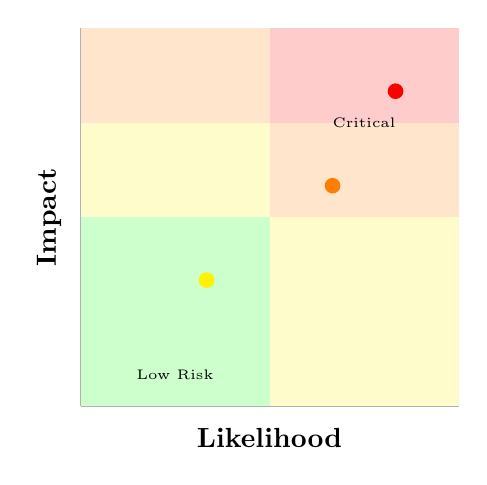
\begin{tikzpicture}[scale=0.8]
            % Draw grid
            \draw[step=1.5cm, black!30, thin] (0,0) grid (6,6);

            % Axes labels
            \node[rotate=90] at (-0.5,3) {\textbf{Impact}};
            \node at (3,-0.5) {\textbf{Likelihood}};

            % Color zones
            \fill[green!20] (0,0) rectangle (3,3);
            \fill[yellow!20] (3,0) rectangle (6,3);
            \fill[yellow!20] (0,3) rectangle (3,4.5);
            \fill[orange!20] (3,3) rectangle (6,4.5);
            \fill[orange!20] (0,4.5) rectangle (3,6);
            \fill[red!20] (3,4.5) rectangle (6,6);

            % Labels
            \node[font=\tiny] at (1.5,0.5) {Low Risk};
            \node[font=\tiny] at (4.5,4.5) {Critical};

            % Example threats (would be populated from registry)
            \node[circle, fill=red, inner sep=2pt] at (5,5) {};
            \node[circle, fill=orange, inner sep=2pt] at (4,3.5) {};
            \node[circle, fill=yellow, inner sep=2pt] at (2,2) {};
        \end{tikzpicture}

        \vspace{5pt}
        \textit{Threat Assessment - Generated: \today}
        \end{minipage}
    };
}

% Annotate node with threat indicator
% Usage: \annotateThreatVector{nodename}{threattype}
% Threat types: ddos, malware, injection, mitm, etc.
\newcommand{\annotateThreatVector}[2]{
    \node[
        rectangle,
        draw=red!70,
        fill=red!10,
        rounded corners=2pt,
        font=\tiny\ttfamily,
        inner sep=2pt,
        anchor=south
    ] at (#1.south) [below=2pt] {
        THREAT: #2
    };
}

% ============================================================================
% COMPLIANCE GAP ANALYSIS
% ============================================================================

% Register compliance requirement
% Usage: \registerComplianceReq{reqid}{standard}{requirement}{status}
% Status: compliant, noncompliant, partial
\newcommand{\registerComplianceReq}[4]{
    \pgfkeys{/security/compliance/#1/standard/.initial={#2}}
    \pgfkeys{/security/compliance/#1/requirement/.initial={#3}}
    \pgfkeys{/security/compliance/#1/status/.initial={#4}}
}

% Generate compliance gap report
% Usage: \generateComplianceGap{x}{y}{standard}
\newcommand{\generateComplianceGap}[3]{
    \node[
        rectangle,
        draw=purple!70,
        fill=white,
        line width=2pt,
        rounded corners=3pt,
        inner sep=10pt,
        anchor=north west,
        font=\small
    ] at (#1,#2) {
        \begin{minipage}{10cm}
        \textbf{\Large Compliance Gap Analysis} \\
        \textbf{Standard:} #3 \\[8pt]

        \textbf{Compliance Status:} \\
        \begin{tabular}{|l|l|l|}
        \hline
        \textbf{Requirement} & \textbf{Status} & \textbf{Gap} \\
        \hline
        Network Segmentation & \textcolor{green}{Compliant} & None \\
        Encryption at Rest & \textcolor{orange}{Partial} & DB encryption \\
        Access Controls & \textcolor{green}{Compliant} & None \\
        Audit Logging & \textcolor{red}{Non-compliant} & Missing logs \\
        Incident Response & \textcolor{orange}{Partial} & No playbooks \\
        \hline
        \end{tabular} \\[8pt]

        \textbf{Recommended Actions:} \\
        \begin{enumerate}
        \item Implement comprehensive audit logging
        \item Enable database encryption
        \item Develop incident response playbooks
        \end{enumerate}

        \textit{Compliance Assessment - Generated: \today}
        \end{minipage}
    };
}

% ============================================================================
% SECURITY HARDENING RECOMMENDATIONS
% ============================================================================

% Generate security hardening checklist
% Usage: \generateHardeningChecklist{x}{y}
\newcommand{\generateHardeningChecklist}[2]{
    \node[
        rectangle,
        draw=blue!70,
        fill=white,
        line width=2pt,
        rounded corners=3pt,
        inner sep=10pt,
        anchor=north west,
        font=\small
    ] at (#1,#2) {
        \begin{minipage}{10cm}
        \textbf{\Large Security Hardening Checklist} \\[8pt]

        \textbf{Network Layer:} \\
        $\square$ Enable firewall rules between zones \\
        $\square$ Implement network segmentation \\
        $\square$ Deploy IDS/IPS on critical paths \\
        $\square$ Enable DDoS protection \\[5pt]

        \textbf{Application Layer:} \\
        $\square$ Patch all known vulnerabilities \\
        $\square$ Enable WAF for web applications \\
        $\square$ Implement rate limiting \\
        $\square$ Use secure protocols (TLS 1.3+) \\[5pt]

        \textbf{Data Layer:} \\
        $\square$ Enable encryption at rest \\
        $\square$ Enable encryption in transit \\
        $\square$ Implement database access controls \\
        $\square$ Regular backup verification \\[5pt]

        \textbf{Monitoring:} \\
        $\square$ Centralized logging \\
        $\square$ SIEM integration \\
        $\square$ Alerting on suspicious activity \\
        $\square$ Regular security audits \\

        \vspace{5pt}
        \textit{Hardening Guide - Generated: \today}
        \end{minipage}
    };
}

% ============================================================================
% SECURITY METRICS DASHBOARD
% ============================================================================

% Generate comprehensive security dashboard
% Usage: \generateSecurityDashboard{x}{y}
\newcommand{\generateSecurityDashboard}[2]{
    \calculateVulnerabilityScore{\vulnscore}
    \calculateAttackSurface{\attacksurf}
    \calculateNetworkHealth{\healthscore}

    \node[
        rectangle,
        draw=black!70,
        fill=white,
        line width=3pt,
        rounded corners=5pt,
        inner sep=15pt,
        anchor=north,
        font=\sffamily,
        drop shadow
    ] at (#1,#2) {
        \begin{minipage}{12cm}
        \centering
        \textbf{\Huge Security Dashboard} \\[10pt]

        \begin{tabular}{|l|r|l|}
        \hline
        \textbf{Metric} & \textbf{Value} & \textbf{Status} \\
        \hline
        Network Health & \healthscore/100 &
            \ifdim\healthscore pt>80pt\relax
                \textcolor{green}{Good}
            \else
                \textcolor{orange}{Fair}
            \fi \\
        Vulnerability Score & \vulnscore &
            \ifdim\vulnscore pt>100pt\relax
                \textcolor{red}{High}
            \else
                \textcolor{green}{Low}
            \fi \\
        Attack Surface & \attacksurf &
            \ifdim\attacksurf pt>100pt\relax
                \textcolor{red}{Large}
            \else
                \textcolor{green}{Small}
            \fi \\
        \hline
        Critical Vulnerabilities & \thecriticalVulns &
            \ifnum\thecriticalVulns>0\relax
                \textcolor{red}{Action Needed}
            \else
                \textcolor{green}{OK}
            \fi \\
        Exposed Services & \theexposedServices &
            \ifnum\theexposedServices>10\relax
                \textcolor{orange}{Review}
            \else
                \textcolor{green}{OK}
            \fi \\
        Validation Errors & \thevalidationErrorCount &
            \ifnum\thevalidationErrorCount>0\relax
                \textcolor{red}{Fix Required}
            \else
                \textcolor{green}{OK}
            \fi \\
        \hline
        \end{tabular} \\[10pt]

        \textbf{Overall Security Posture:}
        \pgfmathsetmacro{\secposture}{(100 - \vulnscore/10)}
        \ifdim\secposture pt>80pt\relax
            \textcolor{green}{\Large STRONG}
        \else
            \ifdim\secposture pt>60pt\relax
                \textcolor{orange}{\Large MODERATE}
            \else
                \textcolor{red}{\Large WEAK}
            \fi
        \fi

        \vspace{5pt}
        \hrule
        \vspace{3pt}
        {\tiny Security Assessment - Generated: \today}
        \end{minipage}
    };
}

% Reset security counters
% Usage: \resetSecurityCounters
\newcommand{\resetSecurityCounters}{
    \setcounter{criticalVulns}{0}
    \setcounter{highVulns}{0}
    \setcounter{mediumVulns}{0}
    \setcounter{lowVulns}{0}
    \setcounter{exposedServices}{0}
    \setcounter{unencryptedConns}{0}
}

% TODO: Advanced security assessment features
% - Automated penetration testing visualization
% - Zero-trust architecture validation
% - Microsegmentation recommendations
% - Security event correlation
% - Threat intelligence integration
% - Ransomware resilience scoring
